\chapter{用于身份识别与认证的协议}

在这一部分,我们关注身份认证和登录问题。考虑甲方希望向乙方表明自己的身份以获取乙方提供的可用资源。他们使用身份识别协议来实现这一目的。识别协议是密码学提供的基本工具之一。我们下面给出几个具体应用场景作为说明,旨在为读者建立一个直观的理解。

\emph{打开一把门锁}。Alice 想通过数字门锁的身份识别,以打开门锁并进入房间。Alice 可以使用一个简单的口令系统,她将电子钥匙插入门锁,如果这个钥匙提供了一个有效的口令,门锁就会打开。与这个场景类似的场景是电脑或者手机上的本地登录界面,当 Alice 想要向设备表明身份来获取访问权时,她可以使用口令来解锁电脑或者手机。

\emph{解锁汽车}。Alice 想要用一个无线硬件钥匙来解锁她的智能汽车,这把钥匙扣能与汽车互动。对手可以窃听无线电信道并记录钥匙扣与汽车之间的一次或若干次通信。尽管如此,对手仍然无法通过这种\emph{窃听攻击}解锁汽车。

\emph{登录银行自动取款机}。Alice 想要使用 ATM 机从自己的账户中提取现金。问题是,她可能正在与一台假的 ATM 机交互。一份来自某个大型ATM设备提供商的报告显示,假 ATM 机正在成为银行业的一个重大威胁:
\begin{quote}
早在 1993 年,就有犯罪团伙在曼彻斯特的一个购物中心安装了一台假的自动柜员机。这种假机器的设计目的并不是直接偷钱,而是在顾客面前假装不能正常工作,同时从试图使用的顾客那里窃取银行卡的信息。
\end{quote}
使用这样的一个假的ATM机,对手就可以与Alice交互并试图窃取她的凭证,并在之后使用该凭证来假冒Alice进行认证。我们称这种对手为\emph{主动}对手。我们的目标是设计识别协议,确保即使是这种主动对手也无法攻破安全系统。

\emph{登录到一个在线银行账户}。Alice 想要访问她的在线银行账户。她的浏览器首先与银行建立了一个安全信道。随后 Alice 通过安全信道运行一个身份识别协议向银行证明自己的身份,比如使用口令,就像之前的例子一样。问题是对手同样可以克隆一个银行的网站来欺骗 Alice,这样 Alice 就会向对手的网站提供自己的信息。这种攻击被称为\textbf{网络钓鱼(phishing)},它是另一个主动攻击的典型例子,对手在与 Alice 交互的过程中扮演一个积极的角色。


对手试图窃取她的凭证,以便以后可以将凭证卖给任何希望冒充 Alice 到真正银行的人。同样,我们的目标是确保即使是网络钓鱼的对手也无法得知 Alice 的有效凭证。我们将在第21.11.1节中更详细地讨论网络钓鱼攻击,并介绍一种潜在的密码学防御手段。

\begin{snote}[身份识别协议 (Identification protocols)。]
身份识别协议在上述所有的场景中都会用到。抽象地讲,身份识别问题涉及到两方,即一个\textbf{证明者 (prover)} 和一个\textbf{验证者(verifier)}。

比如说在ATM的例子中,Alice扮演证明者的角色,而ATM机则扮演验证者的角色。证明者有一个\textbf{证明私钥}$sk$,它能用来说服验证者相信自己的身份。而验证者有一个相应的\textbf{验证密钥}$vk$,它能用来确认证明者的声称。我们有时会把证明者称为人类用户,把验证者称为计算机或服务器。

上面的几个例子也揭示了身份识别协议的三种攻击模型,我们将在接下来的章节中详细讨论这些模型:

\begin{itemize}
    \item \textbf{直接攻击}:门锁和本地登录的例子描述了物理距离上接近的证明者和验证者之间的交互。如果对手无法窃听到交互的内容,那么除了公开的信息之外,对手无法得到任何其他的有效信息,因此对手必须以某种方式在验证者面前冒充证明者。一个简单的口令协议就足以抵御这种直接攻击。
    \item \textbf{窃听攻击}:在无线汽车钥匙的例子中,对手可以窃听无线电信道并获得证明者和验证者之间的若干次交互记录。在这种情况下,简单的口令协议也是不安全的。但是稍微复杂一点的一次性口令协议就能够保证安全。
    \item \textbf{主动攻击}:最后两个例子,也就是假ATM机和假的网上银行,展示了一个更加积极主动的对手。对手在这种场合中试图主动学习一些信息,让它能够在以后的验证过程中冒充证明者。抵御这种主动攻击的身份识别协议往往需要在证明者和验证者之间进行多次交互,我们通常把这种技术称为挑战-应答。
\end{itemize}

当Alice试图登录一台已受感染的计算机时,发生的攻击也属于主动攻击。感染计算机的恶意软件可以展示一个假的登录界面并欺骗Alice与之交互,从而发动主动攻击。以这种方式窃取用户口令的恶意软件被称为\textbf{木马(Trojan horse)}。被盗的口令可以用来冒充Alice登入其他设备。	
\end{snote}

\begin{snote}[验证密钥的保密与公开.]
在一些身份识别协议中,验证者必须将其验证密钥 $vk$ 保密,而另一些协议允许 $vk$ 公开。显然,可以公开 $vk$ 的协议更具优势,因为在这种协议中,即使验证者(比如 ATM 机)被攻破,也不会造成任何损害。
\end{snote}

\begin{snote}[无状态协议与有状态协议.]
理想情况下,在协议设置阶段之后,$vk$和$sk$的值就不会再被修改。但是在某些协议中,$vk$ 和 $sk$ 的值在每次协议执行时都会更新,其中证明者更新 $sk$,验证者更新 $vk$。我们称 $vk$ 和 $sk$ 永远固定的协议为\textbf{无状态}协议,而 $vk$ 和 $sk$ 会被更新的协议为\textbf{有状态}协议。一些有状态协议能够比无状态协议以更低的成本提供更高的安全性。但是有状态协议往往更难使用,因为证明者和验证者需要始终保持正确同步。
\end{snote}

\begin{snote}[单向证明与相互识别.]
在本章中,我们只研究单向的识别问题,即 Bob 希望验证 Alice 的身份。与此相关的另一个话题是\textbf{相互识别},即 Bob 同样也要向 Alice 证明自己的身份。我们将在第21章探讨这部分内容,届时我们会构造能够生成一个共享密钥的相互识别协议。
\end{snote}

\begin{snote}[身份识别协议的安全性和局限性.]
识别协议是为了防止对手在没有 Alice 协助的情况下仿冒 Alice。在定义身份识别协议的安全性时,我们可以允许对手窃听协议通信,甚至直接与 Alice 进行交互。但是,当对手开始尝试冒充 Alice 时,它必须在不与 Alice 通信的情况下进行。在上面的例子里,比如打开门锁的场景,我们给出了一些设定,主要目标就是在Alice不在的时候防止冒充。

然而,身份识别协议并不足以在Alice和远程的参与方(比如Alice的银行)之间建立安全会话。问题在于,身份识别协议很容易受到中间人(MiTM)攻击。假设Alice通过一个不安全的信道与她的银行执行一个身份识别协议,那么如果对手控制了信道,它就可以随意阻止或注入信息。对手等待Alice与她的银行运行识别协议,并将所有协议信息从一方转发到另一方。一旦协议成功完成,对手就可以向银行发送请求,这些请求似乎来自Alice,因此银行会尊重这些请求。实际上,对手利用Alice向银行进行身份验证,然后劫持会话以向银行发送自己的信息。

为了抵抗MiTM攻击,我们可以把识别协议和会话密钥交换协议结合起来,正如我们将在第21章讨论的那样。在Alice和她的银行之间共享会话密钥可以防止对手仿冒Alice注入消息。	
\end{snote}

\section{交互式协议:基本表记}

在具体介绍身份识别协议之前,我们首先需要准确定义\textbf{交互式协议 (interactive protocol)}。

一个交互式协议可以在任意数量的参与方之间进行,但在本文中我们主要关注两方协议。不管有多少参与方,一个协议都可以运行很多次。我们把每一次协议的运行称为\textbf{协议实例(protocol instance)}。

在任意一个协议实例中,每一方都会从初始化设置开始。随着协议的运行,各参与方会发送和接收消息,并更新其本地设置。尽管具体细节因协议不同而各异,但是我们可以使用一个\textbf{交互式协议算法}来对协议实例中各方的计算进行建模。这种算法是一个概率性算法 $I$,它接收元组 $({config}_\mathrm{old}, {data}_\mathrm{in})$ 作为输入,并输出一个新元组 $({config}_\mathrm{new}, {data}_\mathrm{out})$。当某一方开始执行一个协议实例时,它首先需要提供一个\textbf{输入值},这个输入值用于对该参与方的协议实例进行\textbf{初始化设置 (initial configuration)}。当该参与方从网络中收到一个新的消息时,它会调用算法 $I$ 并输入 $({config}_\mathrm{old}, {data}_\mathrm{in})$,其中 ${config}_\mathrm{old}$ 是该方先前的状态,${data}_\mathrm{in}$ 是接收到的消息;$I$ 将会输出元组 $({config}_\mathrm{new}, {data}_\mathrm{out})$,其中 ${config}_\mathrm{new}$ 是该方新的状态,${data}_\mathrm{out}$ 是发出的消息。该方会通过传输信道发送消息给协议的另一参与方。根据协议的要求,上述过程会被反复执行若干次,直到达到某个\textbf{终止设置 (terminal configuration)}。这种终止配置可以指定一个\textbf{输出值},该输出值可以被
该方使用,比如说用于一些更高层的协议中。

一般来说,一个参与方可能会运行多个协议,或同一协议的多个实例。所有这些不同的协议实例的设置都需要单独维护。

\subsection{数学细节}

像往常一样,我们可以使用第2.3节中定义的术语更精确地定义上述概念。除了上面定义的输入,交互式协议算法 $I$ 还会接受一个安全参数 $\lambda$ 和系统参数 $\Lambda$ 作为输入。然而有几个细节值得讨论。

简单起见,我们可以认为一个运行中的协议实例的设置规模是多项式边界的。也就是说,我们可以将设置为一个比特序列,且该序列的长度总是以固定的 $\lambda$ 的多项式为界。这使得我们可以将定义2.8应用于算法$I$。同样,该定义也要求算法的任何输入也同样应是多项式边界的。因此,对于任何多项式边界的输入,算法$I$的输出也同样是多项式边界的。

我们在这里试图解决的问题如下。假设在每一轮之后,设置的大小会增加一倍。几轮之后,设置的大小将会指数爆炸,尽管在每一轮中,计算的时间与当前配置大小成多项式关系。通过坚持要求状态的大小满足多项式边界,我们就可以避免出现指数爆炸的情况。

简单起见,我们还需要坚持协议的轮复杂度 (round complexity)也是多项式边界的。我们主要对执行恒定轮数的协议感兴趣。更一般地,我们希望协议的轮复杂度也是由 $\lambda$ 的固定多项式来约束。这可以通过要求从任何初始配置开始,$I$ 经过多轮迭代后必然达到一个最终状态来实现。
\section{身份认证协议的定义}


我们首先定义图 \ref{fig:18—1} 所示的构成身份识别协议的各个算法。

\begin{figure}
    \centering
    \tikzset{every picture/.style={line width=0.75pt}}   

\begin{tikzpicture}[x=0.75pt,y=0.75pt,yscale=-1,xscale=1]

\draw  [fill={rgb, 255:red, 255; green, 255; blue, 255 }  ,fill opacity=1 ][line width=1.2] [general shadow={fill=black,shadow xshift=2.25pt,shadow yshift=-2.25pt}] (0,60) -- (60,60) -- (60,150) -- (0,150) -- cycle ;
\draw  [fill={rgb, 255:red, 255; green, 255; blue, 255 }  ,fill opacity=1 ][line width=1.2] [general shadow={fill=black,shadow xshift=2.25pt,shadow yshift=-2.25pt}] (250,60) -- (310,60) -- (310,150) -- (250,150) -- cycle ;

\draw  [->]  (140,20) -- (30,55) ;
\draw  [->]  (170,20) -- (280,55) ;

\draw  [<-]  (64,80) -- (250,80) ;
\draw  [->]  (60,105) -- (249,105) ;
\draw  [<-]  (64,130) -- (250,130) ;

\draw  [->]  (280,150) -- (280,190) ;

\draw (30,75) node   [align=left] {证明者};
\draw (280,75) node   [align=left] {验证者};
\draw (155,10) node    {$G$};
\draw (280,193) node [anchor=north] [inner sep=0.75pt]   [align=left] {$\mathsf{accept}$ 或 $\mathsf{reject}$};
\draw (83,34.1) node [anchor=south east] [inner sep=0.75pt]    {$sk$};
\draw (227,34.1) node [anchor=south west] [inner sep=0.75pt]    {$vk$};


\end{tikzpicture}
    \caption{身份认证协议中的证明者与验证者}
    \label{fig:18—1}
\end{figure}

\begin{definition}
一个\textbf{身份识别协议} 是由三个算法构成的三元组 $\mathcal{I}=(G,P,V)$:
\begin{itemize}
    \item $G$ 是一个概率性的\textbf{密钥生成}算法,不接受任何输入,输出一对密钥 $(vk,sk)$,其中 $vk$ 被称为\textbf{验证密钥 (verification key)},$sk$ 被称为\textbf{私钥 (secret key)};
    \item $P$ 是一个交互式协议算法,称为\textbf{证明者 (prover)},接受 $sk$ 作为输入;
    \item $V$ 是一个交互式协议算法,称为\textbf{验证者 (verifier)},接受 $vk$ 作为输入,输出 $\mathsf{accept}$ 或 $\mathsf{reject}$。
\end{itemize}
我们要求,当 $P(sk)$ 和 $V(vk)$ 进行交互时,$V(vk)$ 总是输出 $\mathsf{accept}$。也就是说,对于 $G$ 的所有可能输出 $(vk,sk)$,如果 $P$ 由 $sk$ 初始化,$V$ 由 $vk$ 初始化,那么当 $P$ 和 $V$ 交互结束时,$V$ 输出 $\mathsf{accept}$ 的概率为 $1$。

\end{definition}
\section{口令协议:针对直接攻击的安全性}\label{sec:18-3}

在\textbf{基本口令协议 (Basic Password protocol)}中,证明者的密钥是一个\textbf{口令} $pw$。在该协议中,证明者将 $pw$ 发送给验证者,验证者需要检查 $pw$ 是否是合法的口令。因此,该协议的密钥 $sk$ 就是 $pw$。显然,只有当对手无法窃听证明者和验证者之间的交互时,这个协议才可以被使用。为了完善对基本口令协议的定义,我们还需要指定验证者如何检查给定的口令是否合法。

首先想到的方法是直接将验证者的公钥也定义为 $vk:=pw$,这样验证者只需要检查它从证明者那里收到的口令与 $vk$ 是否相等即可。但是这种简陋的协议显然是有问题的,因为如果验证者被攻破,所有验证者存储的口令都会直接泄露。

为了避免这个问题,我们可以让验证者保存口令的哈希值,而不是口令本身。我们称这个修改后的口令协议为\textbf{版本 1}。我们下面用一种相当理想化的方式来描述这个协议,在该协议中,我们从某个有限的口令空间中随机均匀地选择口令,但实际情况可能并非如此。

\begin{snote}[口令协议版本 1.]
证明者的私钥 $sk$ 是一个从有限口令空间 $\mathcal P$ 中随机均匀选出的口令 $pw$,验证者的公钥 $vk=H(pw)$,其中的哈希函数为 $H:\mathcal{P}\to\mathcal{Y}$。这样,\textbf{口令身份认证协议} $\mathcal{I}_{\rm pwd}=(G,P,V)$ 的定义如下:
\begin{itemize}
    \item $G$:令 $pw\xleftarrow{\rm R}\mathcal{P}$ 并输出 $sk=pw$ 和 $vk=H(pw)$。
    \item 以 $sk=pw$ 为输入的算法 $P$ 及以 $vk=H(pw)$ 为输入的算法 $V$,它们按照以下方式交互:
    \begin{enumerate}
        \item $P$ 将 $pw$ 发送给 $V$;
        \item 如果收到的 $pw$ 满足 $H(pw)=vk$,$V$ 输出 $\mathsf{accept}$,否则输出 $\mathsf{reject}$。
    \end{enumerate}
\end{itemize}

在一个多用户系统中,验证者(服务器)通常会在数据库中维护一张口令映射表,就像图 \ref{fig:18-2} 一样。因此,对服务器的攻击不会泄露出任何的明文口令。

为了分析上述口令协议的安全性,我们下面首先正式定义针对直接攻击的安全性,然后解释为什么上面的协议能够满足这个安全定义。
\end{snote}

\begin{figure}
    \centering
    \includegraphics[width=0.17\linewidth]{figures/chapter18/fig2.png}
    \caption{储存在服务器中的口令文件(版本1)}
    \label{fig:18-2}
\end{figure}

\begin{game}[针对直接攻击安全的身份识别]\label{game:18-1}
对于一个给定的身份识别协议 $\mathcal{I}=(G,P,V)$ 和一个给定对手 $\mathcal{A}$,攻击游戏按照以下方式运行:
\begin{itemize}
    \item 密钥生成阶段。挑战者运行 $(vk,sk)\xleftarrow{\rm R} G()$ 并将 $vk$ 发送给 $\mathcal{A}$。
    \item 仿冒尝试阶段。挑战者与 $\mathcal{A}$ 交互,其中挑战者掌握 $vk$,并按照验证者的算法 $V$ 运行,而对手 $\mathcal{A}$ 扮演证明者的角色,但不一定会诚实执行证明者的算法 $P$(事实上 $\mathcal{A}$ 根本没有获取到私钥 $sk$)。
\end{itemize}
如果 $V$ 在交互结束时输出 $\mathsf{accept}$,我们就称对手 $\mathcal{A}$ 赢得了本游戏。我们定义 $\rm{ID1\mathsf{adv}}[\mathcal{A},\mathcal{I}]$ 为对手 $\mathcal{A}$ 相对 $\mathcal{I}$ 的优势,其值为 $\mathcal{A}$ 赢得本游戏的概率。{\hfill $\square$}
\end{game}

\begin{definition}\label{def:18-2}
如果对于任意有效对手 $\mathcal{A}$,$\rm{ID1\mathsf{adv}}[\mathcal{A},\mathcal{I}]$ 的值都可以忽略不计,我们就称身份识别协议 $\mathcal{I}$ \textbf{对于直接攻击是安全的}。
\end{definition}

请注意,在游戏 \ref{game:18-1} 中,对手 $\mathcal{A}$ 能够获得的是验证密钥 $vk$。因此,一个将明文口令直接存储的简陋口令协议并不满足定义 \ref{def:18-2}。下面的简单定理表明,版本1的协议是安全的。

\begin{theorem}\label{theo:18-1}
如果哈希函数 $H:\mathcal{P}\to\mathcal{Y}$ 是单向的,那么口令协议 $\mathcal{I}_{pwd}$ 针对直接攻击是安全的。
\end{theorem}

\begin{proof}[证明简述]
为了攻击协议 $\mathcal{I}_{pwd}$,对手 $\mathcal{A}$ 必须能够提供一个口令 $pw'$ 使得 $H(pw')=H(pw)$。需要注意的是 $pw'$ 可能与 $pw$ 不同。而能够提供满足上述要求的 $pw'$ 的对手显然已经破坏了 $H$ 的单向性。
\end{proof}

我们可以注意到,针对直接攻击(见攻击游戏 \ref{game:18-1})的安全性事实上是一个非常弱的安全概念。比如说,尽管口令协议 $\mathcal{I}_{pwd}$ 对于直接攻击是安全的,但是对手哪怕能够窃听到协议的一个实例,它显然就丧失了安全性。

\subsection{利用字典攻击破解口令}

口令协议 $\mathcal{I}_{pwd}$ 在实践中被广泛使用,因为它使用起来非常方便。任何人只要记住一个口令 $pw$,就可以参与到协议中来,扮演证明者的角色,并且不需要任何额外的计算设备。问题是,人类生成和记忆随机口令的能力是在太过糟糕。在实践中,被使用的口令通常太短了。更糟糕的是,口令通常根本就不是随机生成的,而是根据一些可预测的信息推导来的。

\begin{figure}
    \centering
    \includegraphics[width=0.6\linewidth]{figures/chapter18/fig3.png}
    \caption{依次列出的2016年中最常见的15个口令}
    \label{fig:18-3}
\end{figure}

图 \ref{fig:18-3} 总结了2016年进行的一项研究的结果,该研究检查了500万个泄露的口令,这些口令大多由北美和西欧的用户持有。数据显示,这些口令与大集合上的均匀分布相去甚远,尤其是有相当比例的口令属于相对较小的常用口令字典。大约4\%的人使用``123456"这个口令,而大约10\%的人使用前25个最常用口令列表中的某一个。图 \ref{fig:18-3} 中的口令列表在一段时间内非常稳定。每年的变化都非常小。

从现在开始,我们使用\textbf{强口令}来表示从一个很大口令空间 $\mathcal{P}$ 中随机均匀选出的口令。只有口令是强口令时,定理 \ref{theo:18-1} 的安全性声明才有效。相对地,\textbf{弱口令}就是指那些从一些常用口令的小字典中按照某个任意分布选取的口令。我们将弱口令的口令空间表示为 $\mathcal{D}$,则必然有 $\mathcal{D}\subseteq\mathcal{P}$。

\subsubsection{在线字典攻击}

假设现在有一个对手怀疑某个用户的口令很弱,属于某个常用口令的小字典 $\mathcal{D}$。那么对手就可以发动一个\textbf{在线字典攻击}:它只需要逐一尝试 $\mathcal{D}$ 中的所有口令,直到找到匹配的口令。为了进一步提升效率,对手可以按照流行程度对 $\mathcal{D}$ 中的元素进行排序,首先尝试更流行的口令。

一个常见的防御在线字典攻击的方法是,在特定用户 ID 或来自特定 IP 地址的登录尝试每两次失败后,就将服务器的响应时间增加一倍。因此在十次登录失败后,下一次尝试的时间就会是正常响应时间的 $32$ 倍。即使一个用户并不能熟记自己的口令,它也不过需要等待一点时间,所以对它来说这种设计的影响并不大。但是对于恶意攻击者来说,通过暴力破解的方式去猜测口令会变得非常困难。

对手为了应对这种反制对策,可以在许多不同的用户名中尝试同一个普通的口令,比如 $\mathtt{123456}$。此外,对手可以利用位于不同 IP 地址的肉机来反制对于单个 IP 地址的登录尝试次数限制。用这种方式对随机账户进行攻击对于一般的对手来说往往已经足够了,他们通常会在地下论坛中交易攻击得到的数据。

非密码学的防御手段对于阻吓这些在线攻击已经很有效了。但是仍然有更具破坏性的攻击,这种攻击也更难阻止。我们将在接下来讨论这种攻击。

\subsubsection{离线词典攻击}\label{subsubsec:18-3-1-2}

攻击者如果破坏了登录服务器,就可以窃取存储在服务器上的口令数据库。这给了攻击者一个大的哈希口里ing列表,每个在该系统注册的用户都有一个口令。

侵入登录服务器的对手可以窃取服务器上存储的口令数据库,攻击者可以借此得到大量哈希后的口令。除了直接破坏服务器外,还有许多其他方法可以获得口令文件。例如一项研究表明,在eBay上购买的二手硬盘可以包含很多有趣的、未被删除的数据,其中就包括口令文件。

现在假设一个对手设法获得了某个用户的验证密钥 $vk=H(pw)$。如果口令 $pw$ 是弱的,并且属于某个常见口令的小字典 $\mathcal{D}$,那么对手就能够发动\textbf{离线字典攻击},它可以这么做:
\begin{equation}\label{eq:18-1}
	\begin{aligned}
		& \text{对每个~}w\in\mathcal{D}:\\
		& \text{~~~~~~~~如果~}H(w)=vk:\\
		& \text{~~~~~~~~~~~~~~~~输出~} w \text{ 并停机}
	\end{aligned}
\end{equation}
如果 $pw$ 在 $\mathcal{D}$ 中,那么依照上述过程,对手迟早能够获取 $pw$,抑或是另一个 $pw'$ 使得 $H(pw')=H(pw)$。

这种离线字典攻击的时间复杂度是 $O(|\mathcal{D}|)$,其中时间单位为对一个输入计算一次$H$的耗时。这种计算完全可以\emph{脱机}运行,不需要与证明者或服务器有任何交互。

\begin{snote}[口令统计.]
2016年,一个名为 CrackStation 的口令破解服务发布了一个大小约为 15 亿的的常用口令词典。经验证据表明,人类生成的口令中有接近 50\% 都在这个列表中。这意味着,每经过约 15 亿次的离线哈希,每两个口令中就有一个能被破解。如果哈希函数 $H$ 是 SHA256,那么现代 GPU 只需要不到一分钟的时间就能够完成破解。由此我们能够得出一个结论:简单地使用 SHA256 对口令进行哈希处理对保护口令数据来说远远不够。

从另一个角度来说,我们可以发现,只包含可打印字符的 8 位字符口令的总数大约是 $95^8 \approx 2^{52}$ 个,这是因为美式键盘上有 95 个可输入字符。使用现代 GPU 阵列对这组口令中的所有单词运行 SHA256 也不过仅仅几天就可以完成。这说明,\emph{所有}8位以下长度口令在服务器被攻破的情况下都是不安全的。
\end{snote}

\begin{snote}[量子离线口令攻击.]
更糟糕的是,一旦有了大规模的量子计算机,上面的穷举搜索攻击将会更加容易。我们在4.3.4节中介绍过,量子计算机可以在 $\sqrt{n}$ 级别的时间内搜索大小为 $n$ 的空间。因此对于 8 位长度的口令空间来说,量子搜索相当于只需要进行 $\sqrt{2^{52}}=2^{26}$ 次哈希计算。这在现代经典计算机上也仅仅需要几秒钟而已。换言之,由于 8 位长度口令在经典计算机上是不能抵抗穷举搜索的,所以一旦我们拥有一台在速度和大小上与当前经典计算机相当的量子计算机,16 位长度的口令也将失去安全保障。我们将在18.4.3节中讨论一些针对该问题防御措施。
\end{snote}

\subsubsection{含预处理的离线字典攻击}

如果对手能够在发动攻击之前对字典 $\mathcal{D}$ 进行预处理,那么上面讨论的离线字典攻击将会更容易发动。一旦获取了哈希后的口令 $vk$,对手就能够立即从字典中查到原始口令 $pw$。具体来说,我们可以将字典攻击分为两个阶段:一个\textbf{预处理阶段},在获取任何哈希口令之前发动;一个\textbf{攻击阶段},针对特定口令$vk$发起攻击。我们的目标是尽量减少攻击阶段破解特定 $vk$ 所需的时间。

一个简单的带有预处理阶段的字典攻击原理如下:
\begin{equation}\label{eq:18-2}
	\begin{aligned}
		& \text{预处理阶段}:\\
		& \text{~~~~~~~~对于每个~}pw\in\mathcal{D}\text{,将~}(pw,H(pw))\text{~加入列表~}L\\
		& \text{针对输入~}vk\text{~的攻击阶段}:\\
		& \text{~~~~~~~~如果在表~}L\text{~中存在一项~}(pw,vk)\text{,则输出~}pw\\
		& \text{~~~~~~~~否则输出~}\mathsf{fail}
	\end{aligned}
\end{equation}
假设我们把对一个口令计算一次$H$的耗时作为时间单位,那么预处理阶段所需要的时间为 $O(|\mathcal{D}|)$级。如果表 $L$ 存储在一个支持常数时间查找的哈希表中,那么攻击阶段将会非常快,耗时仅仅为常数级。

\begin{snote}[批量离线字典攻击.]
一旦完成预处理,攻击者就能利用它快速破解许多哈希口令。具体来说,假设攻击者从一个被攻破的登录服务器中获得了一个大型的哈希口令数据库 $F$,那么现在使用字典 $\mathcal{D}$ 破解 $F$ 中的哈希后口令仅需要:
\begin{equation}
	\begin{aligned}
		& \text{预处理阶段:}O(|\mathcal{D}|)\\
		& \text{攻击阶段:}O(|F|)
	\end{aligned}
\end{equation}
其中 $|F|$ 指 $F$ 中哈希口令的数量。上述批量离线字典攻击的总工作量是 $O(|\mathcal{D}|+|F|)$,这比针对 $F$ 中每一个元素分别单独发起式 \ref{eq:18-1} 的离线字典攻击要快得多,因为后者的总工作量是 $O(|\mathcal{D}|\times |F|)$。

回忆一下,\ref{subsubsec:18-3-1-2} 节中的统计数据表明,对手可以使用 CrackStation 字典找到 $F$ 中近\emph{半数}的口令。因此一旦完成预处理,只需要 $O(|F|)$ 时间就能完成攻击。事实上这种攻击能够使用极少的工作量暴露数百万个被破解的口令。
\end{snote}

\begin{snote}[时空权衡.]
式 \ref{eq:18-2} 所展示的基于预处理的字典攻击要求攻击者建立并存储一个包含大量哈希口令的列表 $L$。然而当字典 $\mathcal{D}$ 是所有 $2^{52}$ 个 8 字符口令的集合时,这个表 $L$ 可能会相当大,存储成本过高。在第18.7节中,我们会介绍一种名为\textbf{彩虹表}的方法,它在预处理阶段构建一个小得多的表$L$,并用它快速破解口令。比如说,在 $n:=|\mathcal{D}|$ 的情况下,该方法能够实现:
\begin{equation*}
	\begin{aligned}
		& \text{表大小:}O(n^{2/3})\\
		& \text{预处理时间:}O(n)\\
		& \text{攻击时间:}O(n^{2/3})
	\end{aligned}
\end{equation*}
表的大小从 $O(n)$ 缩减到 $O(n^{2/3})$ 级别。然而,攻击一个哈希口令的时间从 $O(1)$ 级增长到 $O(n^{2/3})$ 级。换言之,我们用更长的攻击时间换取了表 $L$ 大小的缩减。正因此,这种方法被称为\textbf{时空权衡}。我们通常不讨论预处理阶段的耗时,因为预处理是一个一次性过程,它在攻击开始之前就完成了。

这种时空权衡进一步说明了为什么简单地存储哈希口令是错误的做法。我们将在之后讨论针对性的防御措施。
\end{snote}
\section{使字典攻击更难实施}

当在服务器上存储弱口令的哈希时,离线字典攻击,尤其是基于预处理的离线字典攻击是一种真正的威胁。本节中,我们将讨论一些针对性的技术,这些技术能够使得字典攻击更加困难。

\subsection{公共盐}

上一节中,我们展示了攻击者如何对字典 $\mathcal{D}$ 进行预处理以构建一个速查表 $L$,进而可以快速破解一个或多个哈希后的口令。一种叫做\textbf{加盐(salting)}的简单防御措施就可以反制这种预处理攻击。就算允许攻击者拥有无限时间对 $\mathcal{D}$ 进行预处理,加盐也可以将破解一个哈希口令文件 $F$ 的时间复杂度提升到:
$$
\Omega(|\mathcal{D}|\times |F|)
$$
换言之,加盐可以确保没有任何其他方法的效率优于基于穷举搜索的暴力破解。

加盐的具体做法是在注册新口令时生成一个称为\textbf{盐(salt)}的随机字符串。系统中的每个用户都会被分配一个新的盐,我们可以认为盐是从一个集合 $\mathcal{S}$ 中随机选出的。在实践中,往往 $|\mathcal{S}|=2^{128}$ 就足以满足要求。这个盐会与口令一起被哈希,得到验证密钥 $vk$。盐也会被存储在服务器的口令表中,如图 \ref{fig:18-4} 所示。只有服务器需要知道盐值,用户甚至不需要知道有盐的存在。

\begin{figure}
  \centering
  \includegraphics[width=0.3\linewidth]{figures/chapter18/fig4.png}
  \caption{口令文件(版本2)}
  \label{fig:18-4}
\end{figure}

于是我们就有了新的口令协议,我们称之为\textbf{口令协议版本2},它的运行方式如下:
\begin{itemize}
	\item $G$:令 $pw \xleftarrow{\rm R}\mathcal{P}$,$salt\overset{\rm R}\leftarrow\mathcal{S}$,计算 $y\leftarrow H(pw,salt)$,输出 $sk=pw$ 和 $vk=(salt,y)$。
	\item 以 $sk=pw$ 为输入的算法 $P$ 和以 $vk=(salt,y)$ 为输入的算法 $V$,按如下逻辑交互:
	\begin{enumerate}
		\item $P$ 将 $pw$ 发送给 $V$;
		\item 如果收到的 $pw$ 满足 $H(pw,salt)=y$,$V$ 输出 $\mathsf{accept}$,否则输出 $\mathsf{reject}$。
	\end{enumerate}
\end{itemize}
与版本 1 的描述一样,版本 2 的描述也是相当理想化的,因为我们假设口令 $pw$ 是从空间 $\mathcal{P}$ 中随机均匀选出的,但实际情况远非如此。

现在有了盐的存在,对手可以采取两种策略去攻击文件 $F$ 中的哈希口令:

\begin{itemize}
	\item 第一种策略是使用批量离线字典攻击。问题是,现在预处理阶段需要考虑哈希函数 $H$ 的庞大的输入集合,事实上集合 $\mathcal{D}\times\mathcal{S}$ 中的任何元素都是可能的输入。因此,如果仍然采用式 \ref{eq:18-2} 中的预处理算法,需要准备的预处理表 $L$ 的规模将达到 $|\mathcal{D}|\times|\mathcal{S}|$。这个大小无论如何都是难以生成的,更不要说出村了。因此,式 \ref{eq:18-2} 所介绍的预处理方法不再可行。
	\item 第二种策略是对 $F$ 中的所有口令进行穷举搜索,就像式 \ref{eq:18-1} 中所做的那样。我们已经说明过,穷举搜索的时间复杂度是
	$$O(|\mathcal{D}|\times |F|)$$
\end{itemize}

为了使得没有任何其他方法的效率优于穷举搜索,即上面的第二种策略,盐值空间 $\mathcal{S}$ 需要尽可能大。即使对手采用时空权衡的方法来对$\mathcal{D}\times\mathcal{S}$进行预处理,也同样应该成立。为了推导对 $\mathcal{S}$ 大小的必要约束,我们首先需要更精确地定义在预处理模型中逆转加盐函数的含义。

\begin{snote}[带有预处理的加盐单向函数.]
为了便于定义,我们将对手 $\mathcal{A}$ 拆分成两个独立的对手 $\mathcal{A}_0$ 和 $\mathcal{A}_1$,其中对手 $\mathcal{A}_0$ 拥有无限运行时间,执行预处理阶段。对手 $\mathcal{A}_1$ 能够高效地进行反转攻击。两个对手之间唯一允许的通信是交换一个 $\ell$ 比特的字符串 $L$,其中 $L$ 是预处理阶段的结果。这些概念在下面的定义中得到了体现,该定义将$H$建模为一个随机预言机。
\end{snote}

\begin{definition}\label{def:18-3}
	假设 $H$ 是一个定义在 $(\mathcal{D}\times\mathcal{S},\mathcal{Y})$ 上的哈希函数。我们定义对手 $\mathcal{A}=(\mathcal{A}_0,\mathcal{A}_1)$ 在预处理模型中攻破哈希函数 $H$ 的单向性的优势为 ${\rm OWsp^{ro}\mathsf{adv}}[\mathcal{A},H]$,其大小为对手 $\mathcal{A}$ 赢得下面游戏的概率:
	\begin{itemize}
		\item $\mathcal{A}_0$ 向 $H$ 发起查询并输出一个建议字符串 $L$;
		\item 挑战者随机选择 $(pw,s)\overset{\rm R}\leftarrow\mathcal{D}\times\mathcal{S}$,令 $y=H(pw,s)$,并将 $(L,y,s)$ 发送给 $\mathcal{A}_1$;
		\item $\mathcal{A}_1$ 向 $H$ 发起查询并输出 $pw'\in\mathcal{D}$。当 $H(pw',s)=y$ 时,$\mathcal{A}$ 获胜。
	\end{itemize}
\end{definition}

需要注意的是,对手 $\mathcal{A}_1$ 同时获得了 $L$ 和盐 $s$,而它的目的是找到带有盐 $s$ 的哈希 $y$ 的原象。下面的定理给出了在预处理模型中反转加盐单向函数 $H$ 的时间界限,其中 $H$ 符合随机预言机模型。

\begin{theorem}\label{theo:18-2}
	假设 $H$ 是一个定义在 $(\mathcal{D}\times\mathcal{S},\mathcal{Y})$ 上的哈希函数,$H$ 符合随机预言机模型,且 $|\mathcal{D}|\leq|\mathcal{Y}|$。令 $\mathcal{A}=(\mathcal{A}_0,\mathcal{A}_1)$ 是一个定义 \ref{def:18-3} 中的对手,其中 $\mathcal{A}_0$ 输出一个 $\ell$ 比特的建议字符串 $L$,$\mathcal{A}_1$ 最多能向 $H$ 发起 $Q_{\rm ro}$ 次查询,则有:
	\begin{equation}
	{\rm OWsp^{ro}\mathsf{adv}}[\mathcal{A},H]
	\leq
	O(\frac{\ell\cdot Q_{\rm ro}}{|\mathcal{S}|\cdot |\mathcal{D}|}+\frac{Q_{\rm ro}}{|\mathcal{D}|})	
	\end{equation}
\end{theorem}

该定理表明,如果 $\mathcal{A}$ 在反转 $vk:=y\in\mathcal{Y}$ 时有恒定成功概率,比如 $0.5$,那么他在攻击阶段必须至少花费 $Q_{\rm ro}\geq\Omega({|\mathcal{D}|\cdot|\mathcal{S}|}/{\ell})$ 的时长。因此,为了防止预处理带来的破解性能提升,我们应该令 $|\mathcal{S}|\geq\Omega(\ell)$,这会确保不会有其他方法效率优于穷举搜索。比如说,如果我们假设建议字符串 $L$ 的最大存储空间为 $2^{80}$,那么盐空间应当至少是 $\{0,1\}^{80}$。在实践中,人们通常取 $|\mathcal{S}|:=\{0,1\}^{128}$。

从技术上讲,定理 \ref{theo:18-2} 限定了破解\emph{单个}口令的时间,但并没有限定\emph{批量}离线字典攻击的时间。在这种情况下,攻击者可以尝试一次性破解 $t$ 个口令,其中$t>1$。然而,我们希望该定理可以被推广到批量攻击中,使得约束 $|\mathcal{S}|\geq\Omega(\ell)$ 即使面对批处理场景仍能够有效防止破解。

\begin{snote}[加盐的局限性.]
虽然加盐可以抵御预处理攻击,但它并不能阻止其他攻击。比如说,即使使用了盐,一个选择了弱口令的用户仍然容易受到式 \ref{eq:18-1}  中的那种离线字典攻击。在接下来的内容中,我们将展示如何对离线字典攻击提供进一步的保护。
\end{snote}

\subsection{秘密盐}

通过向人类口令中添加人工熵,我们可以使对手的破解变得更难。想法是从一个小空间 $\mathcal{S}_{\rm p}$ 中再随机挑选一个短字符串,称为\textbf{秘密盐 (secret salt)}或者\textbf{胡椒 (pepper)},并将其也纳入到哈希计算中。但是秘密盐\emph{不会}被记录在口令文件中,因此产生的口令文件如图 \ref{fig:18-5} 所示。

\begin{figure}
  \centering
  \includegraphics[width=0.45\linewidth]{figures/chapter18/fig5.png}
  \caption{口令文件(版本3)}
  \label{fig:18-5}
\end{figure}

为了验证一个口令,服务器只需要遍历秘密盐的所有可能值,直至找到一个能与存储的哈希值匹配的值。依此设计的\textbf{口令协议(版本 3)}按如下方式运行:
\begin{itemize}
	\item $G$:令 $pw\overset{\rm R}\leftarrow\mathcal{P}$,$salt\overset{\rm R}\leftarrow\mathcal{S}$,$pepper\overset{\rm R}\leftarrow\mathcal{S}_p$,$y\leftarrow H(pw,salt,pepper)$,输出 $sk:=pw$ 和 $vk:=(salt,y)$。
	\item 以 $sk=pw$ 为输入的算法 $P$ 及以 $vk=(salt,y)$ 为输入的算法 $V$,按如下逻辑交互:
	\begin{enumerate}
		\item $P$ 将 $pw$ 发送给 $V$;
		\item 对于收到的 $pw$,如果存在 $p\in\mathcal{S}_{\rm p}$ 满足 $H(pw,salt,p)=y$,$V$ 输出 $\mathsf{accept}$,否则输出 $\mathsf{reject}$。
	\end{enumerate}
\end{itemize}

一个典型的设计是将秘密盐空间设置为 $\mathcal{S}_{\rm p}:=\{0,1\}^{12}$。与版本 2 协议相比,这会使得服务器上的口令验证时长变为原来的 $4096$ 倍,但这在现代计算机上仍然只需要不到百分之一秒的时间,因此用户无法察觉到。然而更重要的是,对手现在破解口令文件中的弱口令的难度也增长到了原来的 $4096$ 倍。

秘密盐使离线字典攻击更加困难,因为现在对手必须在 $\mathcal{D}×\mathcal{S}_{\rm p}$ 空间中搜索,而不仅仅是 $\mathcal{D}$。这种技术对用户体验的影响很小。秘密盐增加了用户口令的熵,但并没有迫使用户记住更复杂的口令。

\subsection{慢哈希函数}

保护弱口令的另一种方法是使用慢哈希函数。回顾一下,用 SHA256 这样的哈希函数对口令进行哈希是非常快的,因此 SHA256 也使得离线字典攻击可能发动成功。现在假设服务器使用一个更慢的哈希函数对口令进行哈希,比如该函数处理一个输入需要百分之一秒,这比 SHA256 慢一万倍左右。尽管这对用户体验的影响微乎其微,但是对手这时再想要对字典中的所有项进行哈希的工作量就增大了一万倍。

那么我们如何构造一个慢哈希函数呢?一个直观的方法就是把一个快速哈希函数迭代足够多的次数,直至它变得很慢。具体地,对于一个定义在 $(\mathcal{X},\mathcal{X})$ 上的哈希函数 $H$,我们现在定义:
\begin{equation}\label{eq:18-5}
	H^{(d)}(x)=H(H(H(\cdots(x)\cdots)))
\end{equation}
这样就将 $H$ 迭代了 $d$ 次,可参见第 14.3 节。如果 $d=10000$,那么计算 $H^{(d)}(x)$ 就比计算 $H(x)$ 要多花一万倍的时间。然而这种方法是有问题的,它也不应该被应用到现实的系统中去。原因之一是,函数 $H^{(d)}(x)$ 也比函数 $H(x)$ 容易逆运算 $d$ 倍,参见练习 14.17。我们下面会介绍一个性质更好的函数。首先,我们先对慢哈希函数进行严格的定义。

\begin{definition}
	一个\textbf{基于口令的密钥推导函数(password-based key derivation function, PBKDF)}是这样的一个函数 $H$,其输入是一个口令 $pw\in\mathcal{P}$,一个空间 $\mathcal{S}$ 中的盐,以及一个难度参数 $d\in\mathbb{Z}^{>0}$;其输出是一个值 $y\in\mathcal{Y}$。我们要求函数 $H$ 能由一个运行时间与 $d$ 成正比的算法有效计算。像往常一样,我们称 PBKDF 定义在 $(\mathcal{P},\mathcal{S},\mathcal{Y})$ 上。
\end{definition}

我们会在练习 18.3 中讨论 PBKDF 的安全要求。我们的第一个 PBKDF 的例子,不妨称之为 \textbf{PBKDF1},就基于式 \ref{eq:18-5},其定义为:
$$
{\rm PBKDF1}_H(pw,salt,d)=H^{(d)}(pw,salt)
$$
对于定义在 $(\mathcal{X},\mathcal{X})$ 上的哈希函数 $H$,PBKDF1 定义在 $(\mathcal{P},\mathcal{S},\mathcal{X})$ 上,其中 $\mathcal{X}=\mathcal{P}\times\mathcal{S}$。由于存在练习 14.17 中所介绍的攻击方式,该构造不会被应用在实际的系统中。

\subsubsection{PBKDF2 函数}

一种在实践中被广泛用于构造慢哈希函数的方法被称为PBKDF2。令 $F$ 是一个定义在 $(\mathcal{P},\mathcal{X},\mathcal{X})$ 上的PRF,其中 $\mathcal{X}:=\{0,1\}^n$,那么由之派生出的 PBKDF,不妨用 $\text{PBKDF2}_F$ 表示,它也定义在$(\mathcal{P},\mathcal{X},\mathcal{X})$ 上,并按如下方式工作:
\begin{equation}\label{eq:18-6}
	{\rm PBKDF2}_F(pw,salt,d):=
	\left\{
	\begin{aligned}
		& x_0\leftarrow F(pw, salt)\\
		& \text{for }i=1,\dots,d-1:\\
		& ~~~~~~x_i\leftarrow F(pw,x_{i-1})\\
		& \text{output }y\leftarrow x_0 \oplus x_1 \oplus \cdots \oplus x_{d-1}\in\mathcal{X}
	\end{aligned}
	\right\}
\end{equation}
上面的式 \ref{eq:18-6} 描述了基本版的 PBKDF2,如果需要输出更多比特,对其稍加调整即可。事实上,PBKDF2 能够输出 $\mathcal{X}^b$ 中的一个元素,其中 $1<b<2^{32}$,方法是计算:
\begin{equation}\label{eq:18-7}
{\rm PBKDF2}_F^{(b)}(pw,salt,d):=
\left(
{\rm PBKDF2}_F(pw,salt_1,d),\dots,
{\rm PBKDF2}_F(pw,salt_b,d)
\right)
\in\mathcal{X}^b
\end{equation}
其中所有的$b$个盐都是由最初给定的盐派生而来的,方法是令$salt_i\leftarrow salt\,||\,{\rm bin}(i)$。这里的${\rm bin}(i)$是$i\in\{1,\dots,b\}$的32位二进制字符串表示。

在实践中,PBKDF2 通常使用 HMAC-SHA256 作为底层 PRF。难度 $d$ 的设置取决于项目需求和硬件速度。例如,iOS 10 中的备份钥匙包使用 PBKDF2 来保护,其中 $d$ 的值是一千万。在Windows 10 中,数据保护 API 默认使用 $d = 8000$,但使用 HMAC-SHA512 作为 PRF。

我们会在练习18.2和18.3中更详细地讨论PBKDF2的安全性。

\subsection{慢内存困难哈希函数}

PBKDF2 的一个重要问题是它容易受到并行硬件攻击。我们知道,大部分现代处理器都是基于缓存的,而计算单元只占整个处理器面积的一小部分。因此,一个商用处理器不能对许多输入进行并行 PBKDF2 计算,也不太适合进行离线字典攻击。

更有经验的攻击者通常会在支持高度并行的专用硬件上运行离线字典攻击,比如 GPU,FPGA,甚至是定制芯片。一个定制芯片可以包装超过一百万个 SHA256 计算单元。如果每个单元每秒可以进行一百万次 SHA256 计算,那么一个对手每秒可以在每个芯片上尝试 $10^{12}$ 个口令。即使 PBKDF2 的难度被设置为 $d=10000$,一个由大约 500 个这样的专用芯片组成的农场也能在不到一天的时间内跑完所有 $2^{52}$ 个 8 位口令。这种攻击之所以能够实现,是因为 SHA256 的硬件实现可以做得相当紧凑,所以大量的 SHA256 计算单元可以打包到一个芯片里。

这表明,我们需要的哈希函数 $H$ 应该要求专用硬件实现也需要庞大的片上面积,这样一个芯片就只能容纳几个计算单元,这就极大程度上降低了定制硬件的性能优势。

那么我们如何建立一个具有较大硬件占用面积的哈希函数 $H$?一种方法是确保计算 $H$ 的每一步都需要大量的内存,这将迫使攻击者将芯片上的大部分区域分配给单次哈希求值所需的内存,这就确保了每个芯片只能包含少量的计算电路。

需要大量内存的哈希函数被称为\textbf{内存困难函数}。已经有一些符合要求的内存难度哈希函数,这些函数能够在随机预言机模型下被严格证明是内存困难的。在我们讨论安全问题之前,让我们先看看一个流行的结构,叫做\textbf{Scrypt}。Scrypt是由一个内存容易的哈希函数$h:\mathcal{X}\rightarrow\mathcal{X}$,其中$\mathcal{X}:=\{0,1\}^n$。得到的函数记作$\text{Scrypt}_h$,如图 \ref{fig:18-6} 所示。

\begin{figure}
  \centering
  \includegraphics[width=0.85\linewidth]{figures/chapter18/fig6.png}
  \caption{函数$\text{Scrypt}_h(x_0,d)$}
  \label{fig:18-6}
\end{figure}

在我们的安全分析中,我们将底层哈希函数 $h$ 当作一个随机预言机。在实践中,函数 $h$ 是由 Salsa 20/8 变换衍生出来的,参见3.6节。难度 $d$ 是根据系统的性能需求来设置的。例如我们可以设置一个恰当的 $d$ 使得计算 Scrypt 需要填满整个芯片的存储空间。这会确保计算 Scrypt 不会太慢,但需要大量的内存。

图 \ref{fig:18-6} 是将Scrypt作为一个哈希函数的描述。另一方面,定义在 $(\mathcal{P},\mathcal{X},\mathcal{X})$ 上的Scrypt PBKDF是基于Scrypt哈希构建的,其工作原理如下:
\begin{equation}\label{eq:18-8}
	{\rm ScryptPBKDF}_h(pw,salt,d):=
	\left\{
	\begin{aligned}
		& x_0\leftarrow {\rm PBKDF2}_F(pw,salt,1)\\
		& y\leftarrow \text{Scrypt}_h(x_0,d)\\
		& \text{output }{\rm PBKDF2}_F(pw,y,1)
	\end{aligned}
	\right\}
\end{equation}
其中 $F$ 是一个定义在 $(\mathcal{P},\mathcal{X},\mathcal{X})$ 上的 PRF。在实践中,我们通常使用HMAC-SHA256作为$F$。如有需要,我们也可多次迭代 Scrypt,以使其速度更慢而不增加所需的内存。同样地,通过调整最后一行的PBKDF2的应用,它可以在$b>1$时输出$\mathcal{X}^b$中的一个元素,就像式 \ref{eq:18-7} 那样。

\begin{snote}[Scrypt 是内存困难的吗?]
通过存储 $\mathcal{X}$ 中的 $d+1$ 个元素,Scrypt 函数可以在 $O(d)$ 时间内被计算。Scrypt 哈希的构建步骤创建了一个大小为 $d+1$ 的数组 $(x_0,\dots,x_d)$,随后重复地从该数组中的随机位置读取数据。正因此,一个想要在 $O(d)$ 时间内完成计算的算法必须在内存中保存整个数组 $(x_0,\dots,x_d)$。但这个结论尚需严格证明。

危险的是,时空权衡可能使攻击者尝试牺牲更多的攻击时间来换取更少的内存消耗。这将是毁灭性的,因为减少的内存将允许攻击者将许多 Scrypt 计算单元打包到一个芯片中,而这正是我们想要极力避免的。

在练习18.6中,我们设计了一种针对Scrypt的简单的时空权衡。它表明对于任意的$1<\alpha<d/2$,只需要存储$\lceil d/\alpha\rceil$ 个$\mathcal{X}$中的元素,就可以在$O(\alpha d)$的时间内完成对 Scrypt 的计算。特别地,使用\emph{恒定}空间的Scrypt可以在$O(d^2)$时间内完成计算。然而这种类型的时空权衡并不能帮助对手。对手需要将$\alpha$倍的Scrypt计算单元装入一个芯片中,但每个计算单元的工作难度也变为原来的$\alpha$倍。因此与图 \ref{fig:18-6} 中的Scrypt实现相比,单个芯片的整体吞吐量并没有变化。尽管如此,我们仍然需要证明没有比Scrypt更好的时空权衡方案。

流水线是对内存难度的另一个威胁。假设存在一个算法,它在计算 Scrypt 时仅仅在算法的其中几个步骤中需要使用 $O(d)$ 的内存。如果算法在其余步骤中仅需要使用常数级的内存空间,那么攻击者就可以通过构建流水线来排列多个 Scrypt 计算单元,这些计算单元之间共享一个 $O(d)$ 大小的存储。这样,每个计算单元仅在它需要 $O(d)$ 存储的几个步骤中调用内存,在其他时间可以把存储释放给其他计算单元使用。这样一来,攻击者仍然可以把许多计算单元打包到一个芯片中,只需要共享一个 $O(d)$ 大小的存储阵列即可。为了防止这种形式的流水线,我们还需要证明每一个 Scrypt 实现都需要\emph{在许多计算步骤中}使用到 $O(d)$ 级别的内存。
\end{snote}

\begin{snote}[Scrypt 是内存困难的.]
为了证明 Scrypt 是内存困难的,我们首先需要定义一个安全模型来分析上面讨论的几种障碍。我们下面定义了一个抽象的并行随机预言机模型,其中的算法 $\mathcal{A}$ 能够并行查询多个输入在随机预言机 $h:\mathcal{Y}\to\mathcal{Z}$ 上的输出。

一个\textbf{并行随机预言机算法} $\mathcal{A}$ 将一个 $x\in\mathcal{X}$ 作为输入,并进行一系列的状态转换。在每个状态下,算法 $\mathcal{A}$ 都会向随机预言机 $h$ 发出一组查询,算法在收到查询的所有响应后就会转入下一状态。该过程将不断重复,直至算法终止,此时算法到达最终状态,其中包含算法的输出。所有中间状态都需要被记录,以便跟踪中间状态的大小。

形式上说,算法 $\mathcal{A}$ 实现了一个确定性映射:
$$\mathcal{A}:\mathcal{X}\times\mathcal{S}\times\mathcal{Z}^{\leq p}\to\mathcal{S}\times\mathcal{Y}^{\leq p}$$
其中 $p$ 是正整数,其工作流程如下:
\begin{itemize}
	\item $\mathcal{A}$ 被作为 $\mathcal{A}(x,\varepsilon,\varepsilon)$ 调用,它输出一个 $\mathcal{S}\times\mathcal{Y}^{\leq p}$ 中的元组 $(s_1,\overline y_1)$。这里,$s_1$ 是 $\mathcal{A}$ 的当前状态,$\overline y_1=(y_1,\dots,y_r)$ 是它对随机预言机 $h:\mathcal{Y}\to\mathcal{Z}$ 所发出的第一组并行查询。
	\item 对于 $i=1,\dots,t$,当 $\mathcal{A}$ 输出 $(s_i,\overline y_i)$,$\overline y_1=(y_1,\dots,y_r)\in\mathcal{Y}^{\leq p}$ 时,我们进行如下操作:
	\begin{itemize}
	  \item 并行地调用随机预言机 $h$,计算$\overline z_i\leftarrow (h(y_1),\dots,h(y_r))$,并且
	  \item 重新调用 $\mathcal{A}$ 并计算 $(s_{i+1},\overline y_{i+1})\leftarrow \mathcal{A}(x,s_i,\overline z_i)$。
	\end{itemize}
	\item 最终 $\mathcal{A}$ 输出 $(s,\varepsilon)$,这表示算法终止,输出值为 $s$。
\end{itemize}

算法 $\mathcal{A}$ 在输入 $x\in\mathcal{X}$ 上的运行时间就是 $\mathcal{A}$ 在终止之前被调用的总次数。以这种方式衡量运行时间,我们可以捕捉到一个事实,即硬件实现可以在多点上并行地计算哈希函数$h$。

我们现在记第 $i$ 步输入 $\mathcal{A}$ 的数据为 $st_i:=(s_i,\overline y_i)$,并称 $st_i$ 为 $i$ 时刻的输入状态。对于 $s\in\mathcal{S}$,我们令 $|s|$ 表示 $s$ 的比特位数,类似地,我们令 $|z|$ 表示 $z\in\mathcal{Z}$ 的长度。对于 $\overline z=(z_1,\dots,z_r)\in\mathcal{Z}^{\leq p}$,我们令 $|\overline z|:=\sum_{j=1}^r|z_i|$。那么当 $\mathcal{Z}=\{0,1\}^n$ 时,我们有 $|\overline z|=rn$。最后,我们将输入状态 $st=(s,\overline z)$ 的长度定义为 $|st|:=|s|+|\overline z|$。
\end{snote}

\begin{definition}
	令 $\mathcal{A}$ 是一个以 $\mathcal{X}$ 中元素作为输入的并行随机预言机算法。记$\mathcal{A}$ 对于随机预言机 $h:\mathcal{Y}\to\mathcal{Z}$ 和 $x\in\mathcal{X}$ 的累计存储复杂度为 ${\rm mem}[\mathcal{A},h,x]$,其定义是:
	$${\rm mem}[\mathcal{A},h,x]:=\sum_{i=1}^t|st_i|$$
\end{definition}

图 \ref{fig:18-6} 中对于预言机$h:\mathcal{X}\to\mathcal{X}$,$\mathcal{X}=\{0,1\}^n$计算$\text{Scrypt}_h(x,d)$的算法的累计存储复杂度是$O(nd^2)$。下面的定理将表示,这种设计是最优的。

\begin{theorem}\label{theo:18-3}
	令 $\mathcal{X}=\{0,1\}^n$ 是一个满足 $|\mathcal{X}|$ 为超多项式的空间,$d$ 为一个使得 $2^{-d}$ 可以忽略不计的值。对于所有的并行随机预言机算法 $\mathcal{A}$ 和所有的 $x\in\mathcal{X}$,都有:
	$$
	  {\rm Pr}
	  \left[
	    \mathcal{A}(x,d)={\rm Scrypt}_h(x,d)
	  \right]
      \leq
      {\rm Pr}
      \left[
      {\rm mem}[\mathcal{A},h,(x,d)]\geq\Omega(d^2n)
      \right]+\delta
    $$
    其中 $\delta$ 是一个可以忽略的值。上面的两个概率都基于随机预言机 $h:\mathcal{X}\to\mathcal{X}$的选择。
\end{theorem}

该定理表明,如果 $\mathcal{A}(x,d)$ 以接近 $1$ 的概率输出 ${\rm Scrypt}_h(x,d)$,那么对于几乎所有的 $h$ 的选择,$\mathcal{A}$ 的累计存储复杂度一定是 $\Omega(d^2n)$ 级的。这表明不可能存在一个针对 Scrypt 的时空权衡策略使得其表现比练习18.6更好。如果一个算法以最大 ${dn}/{\alpha}$ 的存储空间计算 Scrypt,其中 $\alpha>1$,那么它的运行时间必然是 $\Omega(d\alpha)$。否则其累计存储复杂度将突破下限。

同样地,不可能存在对 Scrypt 的流水线式攻击。任何在 $O(d)$ 时间内运行的计算 Scrypt 的可行算法必须在整个算法中使用 $\Omega(d\alpha)$ 的内存。否则其累计存储复杂度也将突破下限。

从技术上讲,定理 \ref{theo:18-3} 限定了在\emph{单一}输入下计算Scrypt所需的时间和空间。它并没有限定\emph{批量}离线字典攻击的时间,此时攻击者试图一次对$p>1$个口令计算Scrypt。然而,我们期望该定理可以被推广到批量的设置中:如果一个算法$\mathcal{A}$对$p$个输入正确地计算了Scrypt的概率接近$1$,那么$\mathcal{A}$的累计存储复杂度一定是$\Omega(d^2np)$。这将表明,在$p$个点上计算Scrypt时,不存在针对Scrypt的时空权衡或流水线攻击。

\subsubsection{模糊口令内存困难函数}

虽然Scrypt是一个健全的内存困难的口令哈希函数,但它很容易受到第4.3.2节中讨论的那种侧信道道攻击。

考虑一个登录服务器,其中一个运行中的进程 $P$ 通过 Scrypt 哈希并验证用户的口令。假设对手获得了对该服务器的低权限访问,对手可以在服务器上运行用户级程序但不能破坏进程 $P$,也不能观察到用户的口令明文。然而,利用这种权限,它仍然可以发起一个名为\textbf{缓存计时攻击 (cache timing attack)} 的巧妙攻击方法,这种攻击能够让攻击者了解到 $P$ 访问内存页的顺序。注意,攻击者并不能知道内存页中存储的内容,他只能获取 $P$ 读取页的顺序。

现在,假设对手捕获了一个哈希值 $y$,它是将式 \ref{eq:18-8} 中介绍的Scrypt PBKDF应用于某个带有公共盐的口令 $pw$ 的结果。通常情况下,对手需要发起一个字典攻击,每次尝试都需要大量的时间和\emph{内存}。然而如果对手掌握了进程 $P$ 在计算$pw$的Scrypt哈希时的的内存访问模式,他就可以用很少的内存对 $pw$ 进行字典攻击。

为了说明如何实现攻击,让我们回顾一下图 \ref{fig:18-6} 中所介绍的Scrypt 的实现。算法在第一次执行第 5 步时,需要从数组$(x_0,\dots,x_d)$读取$j$号元素,其中$j={\rm int}(y_0)\mod(d+1)$。

通过观察 $P$ 对内存的访问,对手可以看到算法第一次执行第5步时读取了哪一页的内存,这就给了对手一个 $j$ 的近似值 $j_a$。由于一个内存页中可能存储了多个数组单元,所以对手并没有办法获取 $j$ 的精确值。尽管如此,这个 $j_a$ 也足以使用有限的内存来测试一个可能的口令$pw'$,方法是:
\begin{enumerate}
	\item 按式 \ref{eq:18-8} 计算 $x_0'\leftarrow{\rm PBKDF2}_F(pw',salt,1)$,
	\item 如图 \ref{fig:18-6} 那样计算 $y_0'$,但不存储任何中间值,然后
	\item 测试 $j'\leftarrow{\rm int}(y_0')\mod(d+1)$ 是否与 $j_a$ 接近。
\end{enumerate}

如果测试失败,那么 $pw'$ 就不是正确的口令。这个过程让对手用很少的内存就能过滤掉字典中的大部分候选口令。这样,用户的口令又变得容易受到硬件攻击。

\begin{snote}[一个解决方案.]
这种攻击之所以有效,是因为 Scrypt 的内存访问模式取决于用户的口令。如果我们有一个可证明安全的内存困难哈希函数,其内存访问模式与用户的口令无关,那就更好了。它仍然可以依赖于用户的盐,因为盐不是秘密。这样的函数被称为\textbf{数据模糊内存难度函数}。这种函数的一个例子是 \textbf{Argon2i B},它与 Scrypt 密切相关,但其第一部分的内存访问模式与口令无关,这就消解了上面描述的侧信道攻击。
\end{snote}

\begin{snote}[慢哈希与秘密盐.]
总结本小节,我们观察到秘密盐方法和慢哈希方法都会增加对手的工作负荷。人们可以使用其中的一种方法,但不能两者兼用。慢速内存难度哈希方法的主要好处是,它使定制的硬件攻击难以实施。与快速哈希函数一起使用的秘密盐并不能防止并行硬件攻击,因此慢内存困难哈希比秘密盐更可取。
\end{snote}

\subsection{其他口令管理问题}

\begin{snote}[共同口令问题 (common password problem).]
用户经常在多台机器和多个网站上拥有账户。理想情况下,所有这些服务器都会采取适当的预防措施来防止对手获得口令文件,并对口令进行适当的加盐和哈希,以降低对手获得该文件时的损失。不幸的是,低安全性服务器的设计者可能不会采取与高安全性服务器一样的安全预防措施。这种低安全性的服务器可能更容易被入侵。此外,这种低安全性的服务器可能会存储没有盐的口令哈希,这使批量字典攻击成为可能,并将检索出所有的弱口令。更糟糕的是,有些服务器甚至会在明处存储哈希值,这样对手就会检索出所有的口令,甚至是强口令。因此对手可以侵入一个低安全级别的服务器,并在该服务器上检索到一些,甚至所有的用户 ID/口令,而且这些口令中的一些也很有可能被用在高安全级别的服务中。因此,尽管在高安全性的服务器上采取了所有的预防措施,但该服务器的安全性可能会被一些完全不相关的、低安全性的服务器的不良安全性所破坏。这个问题被称为\textbf{共同口令问题}。

解决共同口令问题的一个标准方案是安装客户端软件,它能将通用口令转换为独有的网站口令,也就是个 "客户端盐"。令 $H$ 是一个哈希函数,如果用户名为 $id$ 的用户的口令是 $pw$,这个口令将在登录时发送给服务器 $id_{\rm server}$。用户的客户端或浏览器在发送前会将口令 $pw$ 转换为 $\widehat{pw}:=H(pw,id,id_{\rm server})$,然后将 $\widehat{pw}$ 发送给服务器。这样,从服务器的角度来看,用户的口令是 $\widehat{pw}$,而从用户的角度来看,口令仍然是 $pw$。这种技术可以保证,即使该用户在许多服务器上使用同一个口令,也不会受到那些没有正确加盐和哈希的服务器的影响。
\end{snote}

\begin{snote}[生物识别技术 (biometrics).]
基于口令的认证的最大困难是用户往往会忘记他们的口令。所有支持电话中的很大一部分都与口令相关的问题有关。因此,一些已部署的系统试图用人类生物识别技术来取代口令,如指纹、视网膜扫描、面容识别和许多其他技术。人们甚至可以使用击键动态,即击键之间的时间长度和按下一个键的时长作为一种生物识别特征。这个想法是使用生物特征作为用户的口令。

虽然生物识别技术相比口令而言有明显的好处,例如用户不会忘记他的指纹,但它有两个明显的缺点:
\begin{itemize}
	\item 生物识别技术通常不是机密的,人们会在他们接触的几乎任何东西上留下他们的指纹;
	\item 生物识别技术是不可逆的,一旦生物识别特征被盗,用户就无法追索。
\end{itemize}
因此,生物识别技术不应该被用作识别用户的唯一手段,只适合作为额外的识别手段(有时被称为第二因素认证)来提高安全性。
\end{snote}
\section{一次性口令:针对窃听攻击的安全性}

\subsection{挑战-应答协议}\label{subsec:18-6-1}

\subsubsection{用公钥$vk$应答挑战}\label{subsubsec:18-6-1-1}
\section{挑战-应答:针对主动攻击的安全性}\label{sec:18-6}
\section{一个有趣的应用:彩虹表}\label{sec:18-7}

令 $h:\mathcal{P}\to\mathcal{Y}$ 是一个随机函数,并设置 $N:=|\mathcal{P}|$。我们来看看计算 $h$ 的逆这个一般的问题。我们假设 $|\mathcal{Y}|\geq N$,因为这是实践中的典型情况。比如说,$\mathcal{P}$ 可能是所有 $8$ 字符口令的集合,而 $\mathcal{Y}=\{0,1\}^{256}$。

令 $pw\overset{\rm R}\leftarrow\mathcal{P}$,并令 $y\leftarrow h(pw)$。显然,对 $\mathcal{P}$ 的所有可能性进行穷举搜索,只要对 $h$ 进行最多 $N$ 次查询,就可以确保找到 $y$ 的原像。在本节中,我们将开发一种更快的算法,它使用一种称作\textbf{彩虹表(rainbow table)}的方法来求取 $h$ 的逆。求逆算法 $\mathcal{A}=(\mathcal{A}_0,\mathcal{A}_1)$ 分两个阶段进行:
\begin{itemize}
	\item 预处理阶段:算法 $\mathcal{A}_0$ 查询 $h$,并输出一张包含 $\ell$ 个 $\mathcal{P}^2$ 中的数对的表 $L$,其中 $\ell$ 是某个正整数。该预处理阶段耗时为 $O(N)$,但它在获知挑战 $y$ 之前已被离线完成。产生的表 $L$ 被称为彩虹表,它必须被妥善储存,以便在第二阶段使用。
	\item 攻击阶段:一旦被赋予一个挑战 $y\in\mathcal{Y}$,$\mathcal{A}_1$ 算法就会以 $\mathcal{A}_1(L,y)$ 的方式被调用,使用 $L$ 快速地找到 $y$ 的逆元。它能以接近 $1$ 的概率输出一个 $h^{-1}(y)$ 中的原像 $pw'$。
\end{itemize}
令 $t$ 为 $\mathcal{A}_1$ 在攻击阶段中的运行时间。下面,我们展示如何在时间 $t$ 内计算 $h$ 的逆,其中:
\begin{equation}\label{eq:18-9}
t\times\ell^2\approx N^2
\end{equation}
举例来说,如果我们可以存储一个大小为 $\ell=N^{2/3}$ 的表 $L$,我们就可以在 $t\approx N^{2/3}$ 的时间内以接近 $1$ 的概率计算 $h$ 的逆,这比在 $\mathcal{P}$ 上进行穷举搜索要快得多。

式 \ref{eq:18-9} 被称作\textbf{时空权衡(time-space tradeoff)}。我们留给表 $L$ 的空间越大,求取 $h$ 的逆的速度就越快。当然,一旦我们有了表 $L$,我们就可以用它来快速地找到许多 $\mathcal{Y}$ 中元素的逆。

正如 \ref{subsubsec:18-3-1-3} 小节所述,彩虹表通常被用于破解未加盐的口令。它们也可以用于从已知的明文-密文对 $\big(m,\,c=E(k,m)\big)$ 中恢复分组密码 $(E,D)$ 的秘钥 $k$。这是因为密钥 $k$ 就是函数 $h(k):=E(k,m)$ 在 $c$ 点处的逆元。如果 $m$ 足够长,或者提供足够多的明文-密文对,那么这个逆元 $k$ 就是唯一的。将此结论应用于 AES-128,我们就可以得到一个大小为 $128\times(2^{128})^{(2/3)}\approx 128\times 2^{85}$ 比特的表 $L$(约 $10$ 亿艾字节),它可以被用来在 $2^{85}$ 的时间内破解 AES。它的耗时在今天来看可能太长,但在几十年后可能会变得可以接受。我们曾在第 \ref{subsubsec:4-2-2-1} 小节中讨论过这种威胁。这种威胁也是迫使人们转向 AES-256 的一个很重要的原因。但是请注意,建立表 $L$ 需要大量(一次性的)工作,即大约 $2^{128}$ 次对 AES-128 的评估。

细心的读者会注意到,式 \ref{eq:18-9} 中的边界在 $\ell=1$ 时相当差,此时,我们有 $t\approx N^2$。这比耗时为 $N$ 的简单穷举搜索还要差得多。这说明,彩虹表算法对于某些 $\ell$ 值来说并不严格。改进时空权衡 \ref{eq:18-9} 是一个长期存在的开放性问题(见练习 \ref{exer:18-7})。

\begin{snote}[Hellman 的基本时空权衡。]
第一个用于求取随机函数的逆的时空权衡是由 Hellman 发明的,它是对 DES 的短密钥设计($56$ 比特)的一个有力批评。Hellman 的方法使用了一个可有效计算的辅助函数 $g:\mathcal{Y}\to\mathcal{P}$,被称为\textbf{还原函数(reduction function)}。它能将 $h$ 的一个 $\mathcal{Y}$ 上的输出``还原"为一个 $\mathcal{P}$ 上的元素。简单起见,我们假设 $g$ 也是一个随机函数。那么,函数 $f(pw):=g(h(pw))$ 就会将 $\mathcal{P}$ 映射到它自身。

预处理算法 $\mathcal{A}_0$ 使用函数 $f:\mathcal{P}\to\mathcal{P}$,它以两个正常数 $\tau$ 和 $\ell$ 为参数。回顾一下,对于 $\tau>0$,函数 $f^{(\tau)}$ 就是定义在 \ref{eq:18-5} 中的 $f$ 的 $\tau$ 次迭代。图 \ref{fig:18-13-a} 直观地展示了算法 $\mathcal{A}_0$ 的工作原理,它运行如下:

\vspace*{10pt}

\hspace*{5pt} 算法 $\mathcal{A}_0$:(预处理 $h$)\\
\hspace*{50pt} 对于 $i=1,\dots,\ell$:\\
\hspace*{75pt} 随机选取 $pw_i\overset{\rm R}\leftarrow\mathcal{P}$\\
\hspace*{75pt} 令 $z_i\leftarrow f^{(\tau)}(pw_i)\in\mathcal{P}$
\hspace*{100pt} // \emph{对 $f$ 进行 $\tau$ 次评估}

\vspace*{5pt}

\hspace*{28.5pt} 输出 $L:=\big\{(pw_1,z_1),\dots,(pw_\ell,z_\ell)\big\}\subseteq\mathcal{P}^2$
\hspace*{37pt} // \emph{输出 $\ell$ 个 $\mathcal{P}^2$ 中的数对}

\vspace*{10pt}

\begin{figure}
  \centering
  \subfigure[Hellman 的基本时空权衡]{
  	  \tikzset{every picture/.style={line width=0.75pt}}

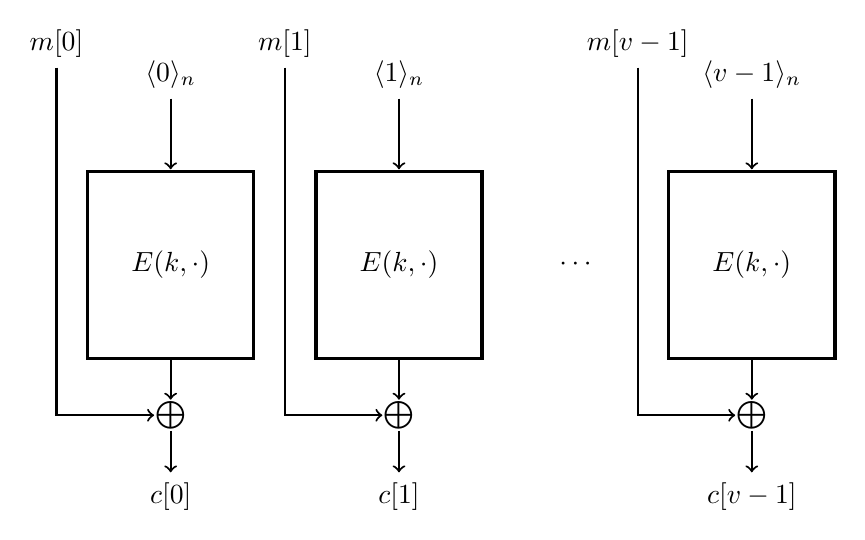
\begin{tikzpicture}[x=0.75pt,y=0.75pt,yscale=-1,xscale=1]

\draw  [line width=1.2]  (30,80) -- (110,80) -- (110,170) -- (30,170) -- cycle ;
\draw  [line width=1.2]  (140,80) -- (220,80) -- (220,170) -- (140,170) -- cycle ;
\draw  [line width=1.2]  (310,80) -- (390,80) -- (390,170) -- (310,170) -- cycle ;

\draw  [->]  (70,45) -- (70,79) ;
\draw  [->]  (180,45) -- (180,79) ;
\draw  [->]  (350,45) -- (350,79) ;
\draw  [->]  (70,170) -- (70,190) ;
\draw  [->]  (70,205) -- (70,225) ;
\draw  [->]  (180,170) -- (180,190) ;
\draw  [->]  (180,205) -- (180,225) ;
\draw  [->]  (350,170) -- (350,190) ;
\draw  [->]  (350,205) -- (350,225) ;
\draw  [->]  (15,30) -- (15,197.5) -- (62,197.5) ;
\draw  [->]  (125,30) -- (125,197.5) -- (172,197.5) ;
\draw  [->]  (295,30) -- (295,197.5) -- (342,197.5) ;

\draw (70,125) node    {$E( k,\cdot )$};
\draw (15,26.6) node [anchor=south] [inner sep=0.75pt]    {$m[ 0]$};
\draw (70.03,228.4) node [anchor=north] [inner sep=0.75pt]    {$c[ 0]$};
\draw (180,125) node    {$E( k,\cdot )$};
\draw (125,26.6) node [anchor=south] [inner sep=0.75pt]    {$m[ 1]$};
\draw (180,228.4) node [anchor=north] [inner sep=0.75pt]    {$c[ 1]$};
\draw (350,125) node    {$E( k,\cdot )$};
\draw (295,26.6) node [anchor=south] [inner sep=0.75pt]    {$m[ v-1]$};
\draw (350,228.4) node [anchor=north] [inner sep=0.75pt]    {$c[ v-1]$};
\draw (265,125) node    {$\cdots $};
\draw (70,197.5) node    {$\bigoplus $};
\draw (180,197.5) node    {$\bigoplus $};
\draw (350,197.5) node    {$\bigoplus $};
\draw (70,41.6) node [anchor=south] [inner sep=0.75pt]    {$\langle 0\rangle _{n}$};
\draw (180,41.6) node [anchor=south] [inner sep=0.75pt]    {$\langle 1\rangle _{n}$};
\draw (350,41.6) node [anchor=south] [inner sep=0.75pt]    {$\langle v-1\rangle _{n}$};

\end{tikzpicture}
  	  \label{fig:18-13-a}
  }
  \subfigure[彩虹表]{
      \tikzset{every picture/.style={line width=0.75pt}}

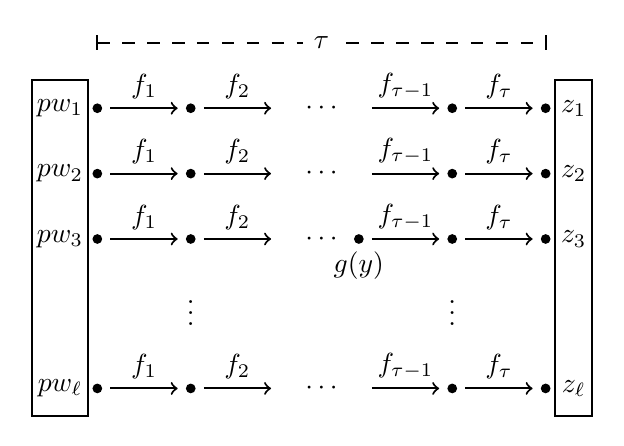
\begin{tikzpicture}[x=0.75pt,y=0.75pt,yscale=-0.9,xscale=0.9]

\draw   (40,40) -- (70,40) -- (70,220) -- (40,220) -- cycle ;
\draw   (320,40) -- (340,40) -- (340,220) -- (320,220) -- cycle ;

\draw  [fill={rgb, 255:red, 0; green, 0; blue, 0 }  ,fill opacity=1 ] (73,55) .. controls (73,53.9) and (73.9,53) .. (75,53) .. controls (76.1,53) and (77,53.9) .. (77,55) .. controls (77,56.1) and (76.1,57) .. (75,57) .. controls (73.9,57) and (73,56.1) .. (73,55) -- cycle ;
\draw  [fill={rgb, 255:red, 0; green, 0; blue, 0 }  ,fill opacity=1 ] (73,90) .. controls (73,88.9) and (73.9,88) .. (75,88) .. controls (76.1,88) and (77,88.9) .. (77,90) .. controls (77,91.1) and (76.1,92) .. (75,92) .. controls (73.9,92) and (73,91.1) .. (73,90) -- cycle ;
\draw  [fill={rgb, 255:red, 0; green, 0; blue, 0 }  ,fill opacity=1 ] (73,125) .. controls (73,123.9) and (73.9,123) .. (75,123) .. controls (76.1,123) and (77,123.9) .. (77,125) .. controls (77,126.1) and (76.1,127) .. (75,127) .. controls (73.9,127) and (73,126.1) .. (73,125) -- cycle ;
\draw  [fill={rgb, 255:red, 0; green, 0; blue, 0 }  ,fill opacity=1 ] (73,205) .. controls (73,203.9) and (73.9,203) .. (75,203) .. controls (76.1,203) and (77,203.9) .. (77,205) .. controls (77,206.1) and (76.1,207) .. (75,207) .. controls (73.9,207) and (73,206.1) .. (73,205) -- cycle ;
\draw  [fill={rgb, 255:red, 0; green, 0; blue, 0 }  ,fill opacity=1 ] (123,55) .. controls (123,53.9) and (123.9,53) .. (125,53) .. controls (126.1,53) and (127,53.9) .. (127,55) .. controls (127,56.1) and (126.1,57) .. (125,57) .. controls (123.9,57) and (123,56.1) .. (123,55) -- cycle ;
\draw  [fill={rgb, 255:red, 0; green, 0; blue, 0 }  ,fill opacity=1 ] (263,55) .. controls (263,53.9) and (263.9,53) .. (265,53) .. controls (266.1,53) and (267,53.9) .. (267,55) .. controls (267,56.1) and (266.1,57) .. (265,57) .. controls (263.9,57) and (263,56.1) .. (263,55) -- cycle ;
\draw  [fill={rgb, 255:red, 0; green, 0; blue, 0 }  ,fill opacity=1 ] (313,55) .. controls (313,53.9) and (313.9,53) .. (315,53) .. controls (316.1,53) and (317,53.9) .. (317,55) .. controls (317,56.1) and (316.1,57) .. (315,57) .. controls (313.9,57) and (313,56.1) .. (313,55) -- cycle ;
\draw  [fill={rgb, 255:red, 0; green, 0; blue, 0 }  ,fill opacity=1 ] (123,90) .. controls (123,88.9) and (123.9,88) .. (125,88) .. controls (126.1,88) and (127,88.9) .. (127,90) .. controls (127,91.1) and (126.1,92) .. (125,92) .. controls (123.9,92) and (123,91.1) .. (123,90) -- cycle ;
\draw  [fill={rgb, 255:red, 0; green, 0; blue, 0 }  ,fill opacity=1 ] (263,90) .. controls (263,88.9) and (263.9,88) .. (265,88) .. controls (266.1,88) and (267,88.9) .. (267,90) .. controls (267,91.1) and (266.1,92) .. (265,92) .. controls (263.9,92) and (263,91.1) .. (263,90) -- cycle ;
\draw  [fill={rgb, 255:red, 0; green, 0; blue, 0 }  ,fill opacity=1 ] (313,90) .. controls (313,88.9) and (313.9,88) .. (315,88) .. controls (316.1,88) and (317,88.9) .. (317,90) .. controls (317,91.1) and (316.1,92) .. (315,92) .. controls (313.9,92) and (313,91.1) .. (313,90) -- cycle ;
\draw  [fill={rgb, 255:red, 0; green, 0; blue, 0 }  ,fill opacity=1 ] (123,125) .. controls (123,123.9) and (123.9,123) .. (125,123) .. controls (126.1,123) and (127,123.9) .. (127,125) .. controls (127,126.1) and (126.1,127) .. (125,127) .. controls (123.9,127) and (123,126.1) .. (123,125) -- cycle ;
\draw  [fill={rgb, 255:red, 0; green, 0; blue, 0 }  ,fill opacity=1 ] (263,125) .. controls (263,123.9) and (263.9,123) .. (265,123) .. controls (266.1,123) and (267,123.9) .. (267,125) .. controls (267,126.1) and (266.1,127) .. (265,127) .. controls (263.9,127) and (263,126.1) .. (263,125) -- cycle ;
\draw  [fill={rgb, 255:red, 0; green, 0; blue, 0 }  ,fill opacity=1 ] (313,125) .. controls (313,123.9) and (313.9,123) .. (315,123) .. controls (316.1,123) and (317,123.9) .. (317,125) .. controls (317,126.1) and (316.1,127) .. (315,127) .. controls (313.9,127) and (313,126.1) .. (313,125) -- cycle ;
\draw  [fill={rgb, 255:red, 0; green, 0; blue, 0 }  ,fill opacity=1 ] (123,205) .. controls (123,203.9) and (123.9,203) .. (125,203) .. controls (126.1,203) and (127,203.9) .. (127,205) .. controls (127,206.1) and (126.1,207) .. (125,207) .. controls (123.9,207) and (123,206.1) .. (123,205) -- cycle ;
\draw  [fill={rgb, 255:red, 0; green, 0; blue, 0 }  ,fill opacity=1 ] (263,205) .. controls (263,203.9) and (263.9,203) .. (265,203) .. controls (266.1,203) and (267,203.9) .. (267,205) .. controls (267,206.1) and (266.1,207) .. (265,207) .. controls (263.9,207) and (263,206.1) .. (263,205) -- cycle ;
\draw  [fill={rgb, 255:red, 0; green, 0; blue, 0 }  ,fill opacity=1 ] (313,205) .. controls (313,203.9) and (313.9,203) .. (315,203) .. controls (316.1,203) and (317,203.9) .. (317,205) .. controls (317,206.1) and (316.1,207) .. (315,207) .. controls (313.9,207) and (313,206.1) .. (313,205) -- cycle ;
\draw  [fill={rgb, 255:red, 0; green, 0; blue, 0 }  ,fill opacity=1 ] (213,125) .. controls (213,123.9) and (213.9,123) .. (215,123) .. controls (216.1,123) and (217,123.9) .. (217,125) .. controls (217,126.1) and (216.1,127) .. (215,127) .. controls (213.9,127) and (213,126.1) .. (213,125) -- cycle ;

\draw  [->]  (82,55) -- (118,55) ;
\draw  [->]  (132,55) -- (168,55) ;
\draw  [->]  (222,55) -- (258,55) ;
\draw  [->]  (272,55) -- (308,55) ;

\draw  [->]  (82,90) -- (118,90) ;
\draw  [->]  (132,90) -- (168,90) ;
\draw  [->]  (222,90) -- (258,90) ;
\draw  [->]  (272,90) -- (308,90) ;

\draw  [->]  (82,125) -- (118,125) ;
\draw  [->]  (132,125) -- (168,125) ;
\draw  [->]  (222,125) -- (258,125) ;
\draw  [->]  (272,125) -- (308,125) ;

\draw  [->]  (82,205) -- (118,205) ;
\draw  [->]  (132,205) -- (168,205) ;
\draw  [->]  (222,205) -- (258,205) ;
\draw  [->]  (272,205) -- (308,205) ;

\draw  [dash pattern={on 4.5pt off 4.5pt}]  (75,20) -- (315,20) ;
\draw [shift={(315,20)}, rotate = 180]  (0,4) -- (0,-4)   ;
\draw [shift={(75,20)}, rotate = 180]   (0,4) -- (0,-4)   ;
\draw  [draw opacity=0][fill={rgb, 255:red, 255; green, 255; blue, 255 }  ,fill opacity=1 ] (185,15) -- (205,15) -- (205,25) -- (185,25) -- cycle ;

\draw (55,55) node    {$pw_{1}$};
\draw (55,90) node    {$pw_{2}$};
\draw (55,125) node    {$pw_{3}$};
\draw (55,205) node    {$pw_{\ell }$};
\draw (195,55) node    {$\cdots $};
\draw (195,90) node    {$\cdots $};
\draw (195,125) node    {$\cdots $};
\draw (195,205) node    {$\cdots $};
\draw (330,55) node    {$z_{1}$};
\draw (330,90) node    {$z_{2}$};
\draw (330,125) node    {$z_{3}$};
\draw (330,205) node    {$z_{\ell }$};
\draw (125,160.03) node    {$\vdots $};
\draw (265,160.03) node    {$\vdots $};
\draw (100,51.6) node [anchor=south] [inner sep=0.75pt]    {$f_{1}$};
\draw (150,51.6) node [anchor=south] [inner sep=0.75pt]    {$f_{2}$};
\draw (240,51.6) node [anchor=south] [inner sep=0.75pt]    {$f_{\tau -1}$};
\draw (290,51.6) node [anchor=south] [inner sep=0.75pt]    {$f_{\tau }$};
\draw (215,130.4) node [anchor=north] [inner sep=0.75pt]    {$g( y)$};
\draw (195,20) node    {$\tau $};
\draw (100,86.6) node [anchor=south] [inner sep=0.75pt]    {$f_{1}$};
\draw (100,121.6) node [anchor=south] [inner sep=0.75pt]    {$f_{1}$};
\draw (100,201.6) node [anchor=south] [inner sep=0.75pt]    {$f_{1}$};
\draw (150,86.6) node [anchor=south] [inner sep=0.75pt]    {$f_{2}$};
\draw (150,121.6) node [anchor=south] [inner sep=0.75pt]    {$f_{2}$};
\draw (150,201.6) node [anchor=south] [inner sep=0.75pt]    {$f_{2}$};
\draw (240,86.6) node [anchor=south] [inner sep=0.75pt]    {$f_{\tau -1}$};
\draw (240,121.6) node [anchor=south] [inner sep=0.75pt]    {$f_{\tau -1}$};
\draw (240,201.6) node [anchor=south] [inner sep=0.75pt]    {$f_{\tau -1}$};
\draw (290,86.6) node [anchor=south] [inner sep=0.75pt]    {$f_{\tau }$};
\draw (290,121.6) node [anchor=south] [inner sep=0.75pt]    {$f_{\tau }$};
\draw (290,201.6) node [anchor=south] [inner sep=0.75pt]    {$f_{\tau }$};


\end{tikzpicture}
  	  \label{fig:18-13-b}
  }
  \caption{时空权衡表,方框内的表项组成了表 $L$。}
  \label{fig:18-13}
\end{figure}

算法 $\mathcal{A}_0$ 建立了 $\ell$ 条水平方向的链,如图 \ref{fig:18-13-a} 所示。对于每条链,表 $L$ 都会记录其起点和终点,其运行时间与 $\tau\times\ell$ 成正比。

接下来,为了使用 $L$ 计算元素 $y\in\mathcal{Y}$ 的逆,我们重复地将 $f$ 作用于 $g(y)$,直到抵达图 \ref{fig:18-13-a} 的最右侧。然后,我们使用 $L$ 跳跃到相关链的起点,并遍历它,直到我们找到 $y$ 的原像。更确切地说,为了计算 $y$ 的逆,我们进行以下操作:

\vspace*{10pt}

\hspace*{5pt} 算法 $\mathcal{A}_1(L,y)$:\\
\hspace*{26pt} 1. \quad 令 $z\leftarrow g(y)\in\mathcal{P}$\\
\hspace*{26pt} 2. \quad 对于 $i=1,\dots,\tau$:\\
\hspace*{26pt} 3. \quad\qquad 如果存在某个 $\widetilde{pw}$ 使得 $(\widetilde{pw},z)\in L$:
\hspace*{20pt} // \emph{如果 $z$ 是一条链的终点} \\
\hspace*{26pt} 4. \quad\qquad\qquad 令 $pw\leftarrow f^{(\tau-i)}(\widetilde{pw})$
\hspace*{73.5pt} // \emph{从起点开始遍历链} \\
\hspace*{26pt} 5. \quad\qquad\qquad 如果 $h(pw)=y$:
\hspace*{87pt} // \emph{如果发现逆元,将其输出} \\
\hspace*{116pt} 输出 $pw$ 并终止\\
\hspace*{26pt} 6. \quad\qquad 令 $z\leftarrow f(z)\in\mathcal{P}$
\hspace*{109pt} // \emph{将链下移} \\
\hspace*{26pt} 7. \quad 输出 $\mathsf{fail}$
\hspace*{168.5pt} // \emph{$g(y)$ 不在任何一条链上}

\vspace*{10pt}

如果图片看起来像图 \ref{fig:18-13-a},那么 $g(y)$ 就会出现在其中一条链的某处,就像图中所展示的那样。一旦我们找到这条链的终点,表 $L$ 就会给出其起点 $pw$。第 $4$ 行的遍历将会给出 $y$ 的逆。求取 $y$ 的逆的总运行时间就是对 $f$ 进行 $\tau$ 次评估和对 $L$ 进行 $\tau$ 次查询的总耗时。

然而,有时情况可能会更复杂一些。图 \ref{fig:18-13-a} 忽略了链之间发生碰撞的可能性,如图 \ref{fig:18-14} 所示。在该图中,第一条链和第二条链发生了碰撞,因为 $f^{(4)}(pw_1)=f^{(6)}(pw_2)$。第二条链和第三条链也发生了碰撞,因为 $f^{(5)}(pw_2)=f^{(7)}(pw_3)$。输入的 $g(y)$ 恰好位于顶部的链上。当我们从 $g(y)$ 开始,沿着顶上这条链移动时,我们首先找到了第三条链的终点 $z_3$,然后是第二条链的终点 $z_2$,最后才是第一条链的终点 $z_1$,后者让我们可以反转 $y$。这就是为什么在第 $5$ 行,我们必须在输出之前检查我们是否已经找到了 $y$ 的逆,以避免误报导致我们遍历错误的链。在图\ref{fig:18-14} 中,$z_3$ 和 $z_2$ 都会引起误报。此外,当 $g(h(pw))=g(y)$ 但 $h(pw)\neq y$ 时,误报也有可能发生,这也是第 $5$ 行检验的另一个原因。
\end{snote}

\begin{snote}[链合并问题。]
尽管 Hellman 的基本方法相当巧妙,但它并不能如描述的那样工作,几乎所有对 $y=h(pw)$ 逆的计算都会失败。让我们来看看原因。要使 $\mathcal{A}_1$ 成功,我们需要确保几乎所有的 $pw\in\mathcal{P}$ 都在至少一条链上。$\mathcal{A}_0$ 能够处理的最大口令有 $\tau\times\ell$ 条。因此,我们至少需要 $\tau\times\ell\geq N$。为了获得最佳性能,我们应该设置 $\tau\times\ell=N$,并希望 $\mathcal{P}$ 中的大多数 $pw$ 都在某条链上。

事实证明,这并不可行。一旦两条链发生碰撞,它们就会合并并且覆盖相同的元素,如图 \ref{fig:18-14} 所示。在建立一张有大量长链的表时,链的合并是不可避免的,并且经常发生。为了说明这个问题的严重性,我们不妨取 $\tau=N^{1/3}$,$\ell=N^{2/3}$,则 $\tau\times\ell=N$。令 $A$ 是预处理过程中遭遇的所有 $\mathcal{P}$ 上元素的集合。如果我们将 $f:\mathcal{P}\to\mathcal{P}$ 建模为一个随机函数,我们就可以证明,集合 $A$ 不太可能包含超过 $o(N)$ 个 $\mathcal{P}$ 上的元素。这意味着,当 $N$ 趋近于无穷大时,$|A|/N$ 趋近于 $0$,因而算法 $\mathcal{A}_1(L,y)$ 对于几乎所有的 $y=h(pw)$ 都会失败。事实上,为了捕获 $\mathcal{P}$ 的一个恒定比例的部分,我们需要 $\ell=\Omega(N)$ 条长度为 $\tau$ 的链。这将使得表 $L$ 的大小也是 $\Omega(N)$,这又使得这种时空权衡失去意义:有一个这么大的表,我们可以在恒定时间内轻而易举地计算 $h$ 的逆。

Hellman 对这个问题的解决方案是建立许多独立的小表,每张表使用不同的还原函数 $g$。每个表包含少量长度为 $τ$ 的链,这确保在单张表内不会发生碰撞。算法 $\mathcal{A}_1$ 分别在每张表中进行搜索,因此,如果有 $m$ 张表的话,运行速度就会慢 $m$ 倍。这样做效果很好,能够达到式 \ref{eq:18-9} 中的约束。然而,另一种被称为彩虹表的解决方案更为简单高效。
\end{snote}

\begin{figure}
  \centering
  \tikzset{every picture/.style={line width=0.75pt}}

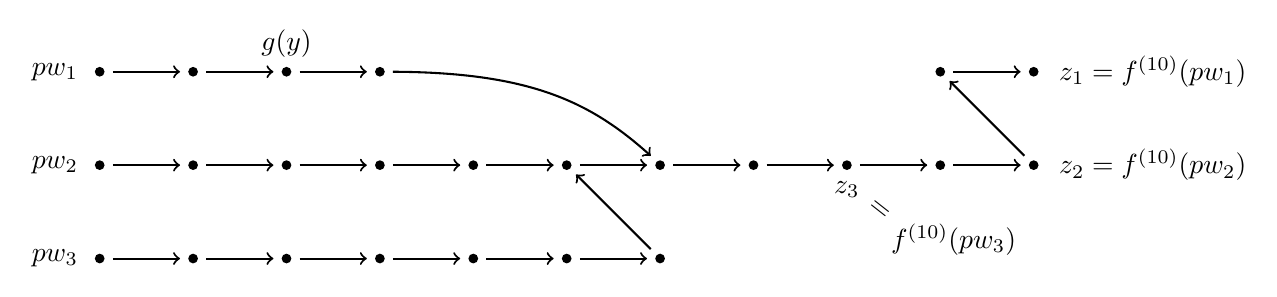
\begin{tikzpicture}[x=0.75pt,y=0.75pt,yscale=-0.9,xscale=0.9]


\draw  [fill={rgb, 255:red, 0; green, 0; blue, 0 }  ,fill opacity=1 ] (38,30) .. controls (38,28.9) and (38.9,28) .. (40,28) .. controls (41.1,28) and (42,28.9) .. (42,30) .. controls (42,31.1) and (41.1,32) .. (40,32) .. controls (38.9,32) and (38,31.1) .. (38,30) -- cycle ;
\draw  [fill={rgb, 255:red, 0; green, 0; blue, 0 }  ,fill opacity=1 ] (88,30) .. controls (88,28.9) and (88.9,28) .. (90,28) .. controls (91.1,28) and (92,28.9) .. (92,30) .. controls (92,31.1) and (91.1,32) .. (90,32) .. controls (88.9,32) and (88,31.1) .. (88,30) -- cycle ;
\draw  [fill={rgb, 255:red, 0; green, 0; blue, 0 }  ,fill opacity=1 ] (138,30) .. controls (138,28.9) and (138.9,28) .. (140,28) .. controls (141.1,28) and (142,28.9) .. (142,30) .. controls (142,31.1) and (141.1,32) .. (140,32) .. controls (138.9,32) and (138,31.1) .. (138,30) -- cycle ;
\draw  [fill={rgb, 255:red, 0; green, 0; blue, 0 }  ,fill opacity=1 ] (188,30) .. controls (188,28.9) and (188.9,28) .. (190,28) .. controls (191.1,28) and (192,28.9) .. (192,30) .. controls (192,31.1) and (191.1,32) .. (190,32) .. controls (188.9,32) and (188,31.1) .. (188,30) -- cycle ;
\draw  [fill={rgb, 255:red, 0; green, 0; blue, 0 }  ,fill opacity=1 ] (38,80) .. controls (38,78.9) and (38.9,78) .. (40,78) .. controls (41.1,78) and (42,78.9) .. (42,80) .. controls (42,81.1) and (41.1,82) .. (40,82) .. controls (38.9,82) and (38,81.1) .. (38,80) -- cycle ;
\draw  [fill={rgb, 255:red, 0; green, 0; blue, 0 }  ,fill opacity=1 ] (88,80) .. controls (88,78.9) and (88.9,78) .. (90,78) .. controls (91.1,78) and (92,78.9) .. (92,80) .. controls (92,81.1) and (91.1,82) .. (90,82) .. controls (88.9,82) and (88,81.1) .. (88,80) -- cycle ;
\draw  [fill={rgb, 255:red, 0; green, 0; blue, 0 }  ,fill opacity=1 ] (138,80) .. controls (138,78.9) and (138.9,78) .. (140,78) .. controls (141.1,78) and (142,78.9) .. (142,80) .. controls (142,81.1) and (141.1,82) .. (140,82) .. controls (138.9,82) and (138,81.1) .. (138,80) -- cycle ;
\draw  [fill={rgb, 255:red, 0; green, 0; blue, 0 }  ,fill opacity=1 ] (188,80) .. controls (188,78.9) and (188.9,78) .. (190,78) .. controls (191.1,78) and (192,78.9) .. (192,80) .. controls (192,81.1) and (191.1,82) .. (190,82) .. controls (188.9,82) and (188,81.1) .. (188,80) -- cycle ;
\draw  [fill={rgb, 255:red, 0; green, 0; blue, 0 }  ,fill opacity=1 ] (38,130) .. controls (38,128.9) and (38.9,128) .. (40,128) .. controls (41.1,128) and (42,128.9) .. (42,130) .. controls (42,131.1) and (41.1,132) .. (40,132) .. controls (38.9,132) and (38,131.1) .. (38,130) -- cycle ;
\draw  [fill={rgb, 255:red, 0; green, 0; blue, 0 }  ,fill opacity=1 ] (88,130) .. controls (88,128.9) and (88.9,128) .. (90,128) .. controls (91.1,128) and (92,128.9) .. (92,130) .. controls (92,131.1) and (91.1,132) .. (90,132) .. controls (88.9,132) and (88,131.1) .. (88,130) -- cycle ;
\draw  [fill={rgb, 255:red, 0; green, 0; blue, 0 }  ,fill opacity=1 ] (138,130) .. controls (138,128.9) and (138.9,128) .. (140,128) .. controls (141.1,128) and (142,128.9) .. (142,130) .. controls (142,131.1) and (141.1,132) .. (140,132) .. controls (138.9,132) and (138,131.1) .. (138,130) -- cycle ;
\draw  [fill={rgb, 255:red, 0; green, 0; blue, 0 }  ,fill opacity=1 ] (188,130) .. controls (188,128.9) and (188.9,128) .. (190,128) .. controls (191.1,128) and (192,128.9) .. (192,130) .. controls (192,131.1) and (191.1,132) .. (190,132) .. controls (188.9,132) and (188,131.1) .. (188,130) -- cycle ;
\draw  [fill={rgb, 255:red, 0; green, 0; blue, 0 }  ,fill opacity=1 ] (238,80) .. controls (238,78.9) and (238.9,78) .. (240,78) .. controls (241.1,78) and (242,78.9) .. (242,80) .. controls (242,81.1) and (241.1,82) .. (240,82) .. controls (238.9,82) and (238,81.1) .. (238,80) -- cycle ;
\draw  [fill={rgb, 255:red, 0; green, 0; blue, 0 }  ,fill opacity=1 ] (288,80) .. controls (288,78.9) and (288.9,78) .. (290,78) .. controls (291.1,78) and (292,78.9) .. (292,80) .. controls (292,81.1) and (291.1,82) .. (290,82) .. controls (288.9,82) and (288,81.1) .. (288,80) -- cycle ;
\draw  [fill={rgb, 255:red, 0; green, 0; blue, 0 }  ,fill opacity=1 ] (338,80) .. controls (338,78.9) and (338.9,78) .. (340,78) .. controls (341.1,78) and (342,78.9) .. (342,80) .. controls (342,81.1) and (341.1,82) .. (340,82) .. controls (338.9,82) and (338,81.1) .. (338,80) -- cycle ;
\draw  [fill={rgb, 255:red, 0; green, 0; blue, 0 }  ,fill opacity=1 ] (238,130) .. controls (238,128.9) and (238.9,128) .. (240,128) .. controls (241.1,128) and (242,128.9) .. (242,130) .. controls (242,131.1) and (241.1,132) .. (240,132) .. controls (238.9,132) and (238,131.1) .. (238,130) -- cycle ;
\draw  [fill={rgb, 255:red, 0; green, 0; blue, 0 }  ,fill opacity=1 ] (288,130) .. controls (288,128.9) and (288.9,128) .. (290,128) .. controls (291.1,128) and (292,128.9) .. (292,130) .. controls (292,131.1) and (291.1,132) .. (290,132) .. controls (288.9,132) and (288,131.1) .. (288,130) -- cycle ;
\draw  [fill={rgb, 255:red, 0; green, 0; blue, 0 }  ,fill opacity=1 ] (338,130) .. controls (338,128.9) and (338.9,128) .. (340,128) .. controls (341.1,128) and (342,128.9) .. (342,130) .. controls (342,131.1) and (341.1,132) .. (340,132) .. controls (338.9,132) and (338,131.1) .. (338,130) -- cycle ;
\draw  [fill={rgb, 255:red, 0; green, 0; blue, 0 }  ,fill opacity=1 ] (388,80) .. controls (388,78.9) and (388.9,78) .. (390,78) .. controls (391.1,78) and (392,78.9) .. (392,80) .. controls (392,81.1) and (391.1,82) .. (390,82) .. controls (388.9,82) and (388,81.1) .. (388,80) -- cycle ;
\draw  [fill={rgb, 255:red, 0; green, 0; blue, 0 }  ,fill opacity=1 ] (438,80) .. controls (438,78.9) and (438.9,78) .. (440,78) .. controls (441.1,78) and (442,78.9) .. (442,80) .. controls (442,81.1) and (441.1,82) .. (440,82) .. controls (438.9,82) and (438,81.1) .. (438,80) -- cycle ;
\draw  [fill={rgb, 255:red, 0; green, 0; blue, 0 }  ,fill opacity=1 ] (488,80) .. controls (488,78.9) and (488.9,78) .. (490,78) .. controls (491.1,78) and (492,78.9) .. (492,80) .. controls (492,81.1) and (491.1,82) .. (490,82) .. controls (488.9,82) and (488,81.1) .. (488,80) -- cycle ;
\draw  [fill={rgb, 255:red, 0; green, 0; blue, 0 }  ,fill opacity=1 ] (538,80) .. controls (538,78.9) and (538.9,78) .. (540,78) .. controls (541.1,78) and (542,78.9) .. (542,80) .. controls (542,81.1) and (541.1,82) .. (540,82) .. controls (538.9,82) and (538,81.1) .. (538,80) -- cycle ;
\draw  [fill={rgb, 255:red, 0; green, 0; blue, 0 }  ,fill opacity=1 ] (488,30) .. controls (488,28.9) and (488.9,28) .. (490,28) .. controls (491.1,28) and (492,28.9) .. (492,30) .. controls (492,31.1) and (491.1,32) .. (490,32) .. controls (488.9,32) and (488,31.1) .. (488,30) -- cycle ;
\draw  [fill={rgb, 255:red, 0; green, 0; blue, 0 }  ,fill opacity=1 ] (538,30) .. controls (538,28.9) and (538.9,28) .. (540,28) .. controls (541.1,28) and (542,28.9) .. (542,30) .. controls (542,31.1) and (541.1,32) .. (540,32) .. controls (538.9,32) and (538,31.1) .. (538,30) -- cycle ;


\draw  [->]  (47,30) -- (83,30) ;
\draw  [->]  (97,30) -- (133,30) ;
\draw  [->]  (147,30) -- (183,30) ;
\draw  [->]  (497,30) -- (533,30) ;

\draw  [->]  (47,80) -- (83,80) ;
\draw  [->]  (97,80) -- (133,80) ;
\draw  [->]  (147,80) -- (183,80) ;
\draw  [->]  (197,80) -- (233,80) ;
\draw  [->]  (247,80) -- (283,80) ;
\draw  [->]  (297,80) -- (333,80) ;
\draw  [->]  (347,80) -- (383,80) ;
\draw  [->]  (397,80) -- (433,80) ;
\draw  [->]  (447,80) -- (483,80) ;
\draw  [->]  (497,80) -- (533,80) ;

\draw  [->]  (47,130) -- (83,130) ;
\draw  [->]  (97,130) -- (133,130) ;
\draw  [->]  (147,130) -- (183,130) ;
\draw  [->]  (197,130) -- (233,130) ;
\draw  [->]  (247,130) -- (283,130) ;
\draw  [->]  (297,130) -- (333,130) ;

\draw  [->]  (335,125) -- (295,85) ;
\draw  [->]  (535,75) -- (495,35) ;

\draw  [->]  (197,30) .. controls (270.33,30.33) and (302.67,46) .. (335,75) ;

\draw (2,30) node [anchor=west] [inner sep=0.75pt]    {$pw_{1}$};
\draw (2,80) node [anchor=west] [inner sep=0.75pt]    {$pw_{2}$};
\draw (2,130) node [anchor=west] [inner sep=0.75pt]    {$pw_{3}$};
\draw (140,24) node [anchor=south] [inner sep=0.75pt]    {$g( y)$};
\draw (440,87) node [anchor=north] [inner sep=0.75pt]    {$z_{3}$};
\draw (552,30) node [anchor=west] [inner sep=0.75pt]    {$z_{1} =f^{( 10)}( pw_{1})$};
\draw (552,80) node [anchor=west] [inner sep=0.75pt]    {$z_{2} =f^{( 10)}( pw_{2})$};
\draw (462,120) node [anchor=west] [inner sep=0.75pt]    {$f^{( 10)}( pw_{3})$};
\draw (454,96) node [anchor=north west][inner sep=0.75pt]  [rotate=-38.18]  {$=$};


\end{tikzpicture}
  \caption{一个链碰撞实例,三条链的长度都是 $10$}
  \label{fig:18-14}
\end{figure}

\begin{snote}[彩虹表。]
链合并问题的一个优雅的解决方案是为图 \ref{fig:18-13-a} 的每一列 $i=1,\dots,\tau$ 使用不同的还原函数 $g_i:\mathcal{Y}\to\mathcal{P}$。和之前一样,令 $f_i(pw)= g_i(h(pw))$。预处理算法 $\mathcal{A}_0$ 现在执行图 \ref{fig:18-13-b} 中的流程。它输出一张与之前相同的表 $L$,该表包含每条链的起点和终点。如果把每条链染上不同的颜色,然后将它们略微向上弯曲,图片看起来就像是一道彩虹,这就是它名字的由来。

在每一列中使用不同的函数 $f_i$ 的意义在于,链的碰撞不一定会导致链的合并。只有当两条链在完全相同的索引处发生碰撞时,它们才会合并。这使得链合并的概率大大降低(见练习 \ref{exer:18-18})。此外,如果一条以 $pw$ 为起点的链恰好与一条以 $pw'$ 为起点的链合并,这两条链的终点 $z$ 和 $z'$ 也会是相等的。预处理算法 $\mathcal{A}_0$ 可以很容易地检测到这种重复的终点,并丢弃掉其中的一条链。最终的结果是,我们可以设定 $\tau=N^{1/3}$,$\ell=N^{2/3}$,并在预处理过程中捕获 $\mathcal{P}$ 的一个恒定比例的部分。

现在,想要用表 $L$ 计算元素 $y\in\mathcal{Y}$ 的逆,注意到,如果 $g(y)$ 包含在图 \ref{fig:18-13-b} 的倒数第二列中,$f_\tau(g(y))$ 就是 $L$ 中某条链的终点;如果 $g(y)$ 包含在图的倒数第三列中,$f_{\tau}f_{\tau-1}(g(y))$ 就是 $L$ 中某条链的终点,以此类推。这就为我们提供了下面这个使用 $L$ 计算 $y$ 的逆的算法:

\vspace*{10pt}

\hspace*{5pt} 算法 $\mathcal{A}_1(L,y)$:\\
\hspace*{26pt} 1. \quad 令 $z\leftarrow g(y)\in\mathcal{P}$\\
\hspace*{26pt} 2. \quad 对于 $i=\tau-1,\dots,0$:\\
\hspace*{26pt} 3. \quad\qquad 如果存在某个 $\widetilde{pw}$ 使得 $(\widetilde{pw},z)\in L$:
\hspace*{40pt} // \emph{如果 $z$ 是一条链的终点} \\
\hspace*{26pt} 4. \quad\qquad\qquad 令 $pw\leftarrow f_i\big(\cdots f_2(f_1(\widetilde{pw}))\cdots\big)$
\hspace*{43pt} // \emph{从起点开始遍历链} \\
\hspace*{26pt} 5. \quad\qquad\qquad 如果 $h(pw)=y$:
\hspace*{107pt} // \emph{如果发现逆元,将其输出} \\
\hspace*{116pt} 输出 $pw$ 并终止\\
\hspace*{26pt} 6. \quad\qquad 令 $z\leftarrow f_{\tau}\big(f_{\tau-1}(\cdots f_{i+1}(g(y))\cdots)\big) \in\mathcal{P}$
\hspace*{25pt} // \emph{检查 $g(y)$ 是否在第 $i$ 列上} \\
\hspace*{26pt} 7. \quad 输出 $\mathsf{fail}$
\hspace*{188.5pt} // \emph{$g(y)$ 不在任何一条链上}

\vspace*{10pt}

\noindent
该算法的大部分工作是在第 $6$ 行完成的。在第一次迭代中,该行评估了一次 $f$,在第二次迭代中评估了两次,以此类推。总的来说,第 $6$ 行导致最坏情况下的工作量是 $1+2+\cdots+\tau=\tau(\tau+1)/2\approx\tau^2/2$。因此,$\mathcal{A}_1$ 的最大运行时间是 $t:=\tau^2/2$。为了捕获大部分的 $\mathcal{P}$,我们需要 $\tau\times\ell\geq N$,而由于 $\tau=(2t)^{1/2}$,我们可得:
\[
\ell\times(2t)^{1/2}\geq N
\]
将两边同时平方,我们可得 $\ell^2\times t\geq N^2/2$,这就与式 \ref{eq:18-9} 中承诺的时空权衡一致。还需要注意的是,算法 $\mathcal{A}_1$ 最多只能对表 $L$ 进行 $\tau$ 次查找。
\end{snote}

\begin{snote}[实践中的彩虹表。]
许多流行的哈希函数的彩虹表都是现成的。它们被设计成可以与一个叫做 \textbf{RainbowCrack} 的程序配合使用。比如说,有一张大小为 460 GB 的 SHA1 彩虹表,它可以寻找字母表 \texttt{ascii-32-95} 中所有 $8$ 字符口令的原像。这个字母表包含了美国标准键盘上的所有 $95$ 个字符。该表的成功率接近97\%,而且任何人都可以免费下载它。在 GPU 上,使用该表破解一个 $8$ 字符的 SHA1 哈希口令仅需大约一个小时。
\end{snote}

\begin{snote}[扩展。]
尽管彩虹表旨在计算随机函数的逆,但 Fiat 和 Naor 的另一个算法给出了计算任意函数 $h:\mathcal{P}\to\mathcal{Y}$ 的逆的时空权衡 \cite{fiat1991rigorous}。他们的时空权衡满足 $\ell^2t\geq\lambda N^3$,这意味着,为了在 $t$ 时间内以 $1/2$ 的概率计算函数 $h$ 的逆,他们的预处理算法必须生成一张大小约为 $(\lambda N^3/t)^{1/2}$ 的表。这里,$\lambda$ 是 $h$ 的碰撞概率,定义为 $\lambda:=\Pr[h(x)=h(y)]$,其中 $x,y\overset{\rm R}\leftarrow\mathcal{P}$。当 $h$ 是一个随机函数,并且 $|\mathcal{Y}|\gg|\mathcal{P}|$ 时,我们有 $\lambda=1/N$,这就恢复了式 \ref{eq:18-9} 中的约束。
\end{snote}
\section{一个有趣的应用:强化口令存储}
\section{笔记}\label{sec:18-9}

要增加的文献引用。
\section{练习}

\begin{exercise}\label{exer:18-1}
\end{exercise}

\begin{exercise}\label{exer:18-2}
\end{exercise}

\begin{exercise}\label{exer:18-3}
\end{exercise}

\begin{exercise}\label{exer:18-4}
\end{exercise}

\begin{exercise}\label{exer:18-5}
\end{exercise}

\begin{exercise}\label{exer:18-6}
\end{exercise}

\begin{exercise}\label{exer:18-7}
\end{exercise}

\begin{exercise}\label{exer:18-8}
\end{exercise}

\begin{exercise}\label{exer:18-9}
\end{exercise}

\begin{exercise}\label{exer:18-10}
\end{exercise}

\begin{exercise}\label{exer:18-11}
\end{exercise}

\begin{exercise}\label{exer:18-12}
\end{exercise}

\begin{exercise}\label{exer:18-13}
\end{exercise}

\begin{exercise}\label{exer:18-14}
\end{exercise}

\begin{exercise}\label{exer:18-15}
\end{exercise}

\begin{exercise}\label{exer:18-16}
\end{exercise}

\begin{exercise}\label{exer:18-17}
\end{exercise}

\begin{exercise}\label{exer:18-18}
\end{exercise}

\begin{exercise}\label{exer:18-19}
\end{exercise}

\begin{exercise}\label{exer:18-20}
\end{exercise}
